%%%%%%%%%%%%%%%%%%%%%%%%%%%%%%%%%%%%%%%%%%%%%%%%%%%
%
%  New template code for TAMU Theses and Dissertations starting Fall 2012.  
%  For more info about this template or the 
%  TAMU LaTeX User's Group, see http://www.howdy.me/.
%
%  Author: Wendy Lynn Turner 
%	 Version 1.0 
%  Last updated 8/5/2012
%
%%%%%%%%%%%%%%%%%%%%%%%%%%%%%%%%%%%%%%%%%%%%%%%%%%%

%%%%%%%%%%%%%%%%%%%%%%%%%%%%%%%%%%%%%%%%%%%%%%%%%%%%%%%%%%%%%%%%%%%%%%
%%                           APPENDIX - DSA
%%%%%%%%%%%%%%%%%%%%%%%%%%%%%%%%%%%%%%%%%%%%%%%%%%%%%%%%%%%%%%%%%%%%%

\chapter{\uppercase {Addendum to Chapter 4}}
\label{sec::appendix_DSA}

In this appendix, we will perform some additional analysis of the MIP diffusion form. First, we provide greater implementation details for Fourier Analysis in Section \ref{sec::App_DSA_fourier}. Then, we provide some example Fourier Analysis for the 1D MIP DSA scheme in Section \ref{sec::App_DSA_resutls}. We conclude with a comparison between the MIP and Modified Four-Step (M4S) DSA schemes in Section \ref{sec::App_DSA_M4S}.

%%%%%%%%%%%%%%%%%%%%%%%%%%%%%%%%%%%%%%%%%%%%%%%%%%%
%%%%%%%%%%%%%%%%%%%%%%%%%%%%%%%%%%%%%%%%%%%%%%%%%%%
%%%   Section - 1D
%%%%%%%%%%%%%%%%%%%%%%%%%%%%%%%%%%%%%%%%%%%%%%%%%%%
%%%%%%%%%%%%%%%%%%%%%%%%%%%%%%%%%%%%%%%%%%%%%%%%%%%
\section{Extended Fourier Analysis Implementation for MIP in 1D}
\label{sec::App_DSA_fourier}

In this section, we give greater detail on how to implement discretized Fourier Analysis through the use of a 1D example. The 1D, isotropic scattering, continuous transport equation is given by

\begin{equation}
\label{eq::App_DSA_1D_transport_eq}
\mu \frac{d }{d x} \psi (x,\mu) + \sigma_t (x) \psi(x,\mu) = \frac{\sigma_s (x)}{2} \phi(x) + \frac{Q(x)}{2}.
\end{equation}

\noindent If we define a 1D angular quadrature, $\{  \mu_m, w_m \}_{m=1}^M$, suppress the spatial and angular parameters and apply SI, we can rewrite Eq. (\ref{eq::App_DSA_1D_transport_eq}) into

\begin{equation}
\label{eq::App_DSA_1D_transport_discangle}
\mu_m \frac{d }{d x} \psi_m^{(k+1/2)} + \sigma_t \psi_m^{(k+1/2)} = \frac{\sigma_s }{2} \phi^{(k)}  + \frac{Q}{2},
\end{equation}

\noindent where

\begin{equation}
\label{eq::App_DSA_1D_angint}
\phi^{(k)} = \sum_{m=1}^M w_m \psi_m^{(k)},
\end{equation}

\noindent and we assume constant cross sections and a constant isotropic source. Applying a spatial discretization, we can express Eq. (\ref{eq::App_DSA_1D_transport_discangle}) in operator notation as 

\begin{equation}
\label{eq::App_DSA_1D_transport_ops}
{\bf L} \Psi^{(k+1/2)} = \frac{1}{2} {\bf S} \Phi^{(k)}  + \frac{1}{2} {\bf Q}.
\end{equation}

\noindent If we perform a transport sweep and integrate over the angular quadrature, then we can write Eq. (\ref{eq::App_DSA_1D_transport_ops}) in terms of only the scalar fluxes as

\begin{equation}
\label{eq::App_DSA_1D_transport_phi_ops}
\begin{aligned}
 \Phi^{(k+1/2)} &= \frac{1}{2} {\bf D} {\bf L}^{-1} {\bf S} \Phi^{(k)}  + \frac{1}{2} {\bf D} {\bf L}^{-1} {\bf Q}. \\
 \Phi^{(k+1/2)} &= {\bf T}\Phi^{(k)} + {\bf b}
\end{aligned}.
\end{equation}

\noindent In Eq. (\ref{eq::App_DSA_1D_transport_phi_ops}), ${\bf T}=\frac{1}{2} {\bf D} {\bf L}^{-1} {\bf S}$ and ${\bf b} = \frac{1}{2} {\bf D} {\bf L}^{-1} {\bf Q}$.

We now give the low-order diffusion equation for the transport error as 

\begin{equation}
\label{eq::App_DSA_1D_diff_eq}
- \frac{d}{dx} D \frac{d }{dx} \delta \phi^{(k+1/2)}+ \sigma_a \delta \phi^{(k+1/2)} = \sigma_s \left(  \phi^{(k+1/2)} - \phi^{(k)} \right) ,
\end{equation}

\noindent where the corresponding discretized operator notation is

\begin{equation}
\label{eq::App_DSA_1D_diff_ops}
{\bf A} \delta \Phi^{(k+1/2)} = {\bf S}\left( \Phi^{(k+1/2)} -  \Phi^{(k)}   \right) .
\end{equation}

\noindent Solving for the correction gives

\begin{equation}
\label{eq::App_DSA_1D_diff_corr}
 \delta \Phi^{(k+1/2)} = {\bf A}^{-1} {\bf S}\left( \Phi^{(k+1/2)} -  \Phi^{(k)}   \right) .
\end{equation}

\noindent We now express the SI+DSA iteration as the following:

\begin{equation}
\label{eq::App_DSA_1D_iter}
\begin{aligned}
 \Phi^{(k+1)} &= \Phi^{(k+1/2)} +   \delta \Phi^{(k+1/2)}\\
 &= {\bf T}\Phi^{(k)} + {\bf b} +  {\bf A}^{-1} {\bf S}\left( \Phi^{(k+1/2)} -  \Phi^{(k)}   \right) \\
 &= {\bf T}\Phi^{(k)} + {\bf b} +  {\bf A}^{-1} {\bf S}\left( {\bf T}\Phi^{(k)} + {\bf b} -  \Phi^{(k)}   \right) \\
  &= \left[  {\bf T} + {\bf A}^{-1} {\bf S}\left( {\bf T} -  {\bf I} \right)  \right] \Phi^{(k)} + \left( {\bf I} +  {\bf A}^{-1} {\bf S}  \right){\bf b}
\end{aligned}
\end{equation}

\noindent Therefore, our FA iteration matrix to analyze is $\left[  {\bf T} + {\bf A}^{-1} {\bf S}\left( {\bf T} -  {\bf I} \right)  \right]$. We expand this iteration matrix back out and denote the terms that will require the Fourier transformation with the tilde, $\tilde{}$, to give

\begin{equation}
\label{eq::App_DSA_1D_FA_mat}
\frac{1}{2} {\bf D} \tilde{{\bf L}}^{-1} \tilde{{\bf S}} + \tilde{{\bf A}}^{-1} \tilde{{\bf S}}\left( \frac{1}{2} {\bf D} \tilde{{\bf L}}^{-1} \tilde{{\bf S}} -  {\bf I} \right).
\end{equation}

\noindent Therefore, all that remains is to define each of these terms in terms of the appropriate elementary matrices and phase transformation matrices.

For this analysis, we will only use a single mesh cell. It will have a cell width of $h$ which gives the physical domain of $[0,h]$. Using the 1D LD basis functions, the cell-wise elementary matrices for the mass, stiffness, and gradient matrices for a cell of width $h$ are

\begin{equation}
\label{eq::App_DSA_MIP_1D_cell_matrices}
\begin{aligned}
	\mathbb{M} =& \frac{h}{6}
	\left[ \begin{array}{cc}
	2 & 1 \\
	1 & 2 
	\end{array} \right] ,\\
	\mathbb{K} =& \frac{1}{h}
	\left[ \begin{array}{cc}
	1 & -1 \\
	-1 & 1 
	\end{array} \right] ,\\
	\mathbb{S} =& \frac{1}{2}
	\left[ \begin{array}{cc}
	-1 & -1 \\
	 1 & 1 
	\end{array} \right] ,
\end{aligned}
\end{equation}

\noindent respectively. The values of the basis functions at the left face and right face are given by

\begin{equation}
\label{eq::App_DSA_MIP_1D_facemass_matrices}
\begin{aligned}
	\mathbb{E}_L =& 
	\left[ \begin{array}{c}
	1  \\
	0 
	\end{array} \right] ,\\
	\mathbb{E}_R =& 
	\left[ \begin{array}{c}
	0  \\
	1
	\end{array} \right] ,
\end{aligned}
\end{equation}

\noindent respectively. Likewise, the gradients of the basis functions at the left face and the right face are given by

\begin{equation}
\label{eq::App_DSA_MIP_1D_facegrad_matrices}
\begin{aligned}
	\mathbb{G}_L =& \frac{1}{h}
	\left[ \begin{array}{c}
	-1  \\
	1 
	\end{array} \right] ,\\
	\mathbb{G}_R =& \frac{1}{h}
	\left[ \begin{array}{c}
	-1  \\
	1
	\end{array} \right] ,
\end{aligned}
\end{equation}

\noindent respectively.

Now, we provide the simple definitions of the Fourier phase transformation matrices. Recall that when the matrix coupling is occurring across a boundary, the periodic boundaries enforce that the degrees of freedom from the other side of the domain be used. However, the Fourier phase that is used is that of the virtual cell just on the other side of the domain (we can view these virtual cells as ghost cells). Therefore, the ghost cell to the left of the domain spans $[-h,0]$, and the ghost cell to the right of the domain spans $[h,2h]$. We can write the phase matrices for inside the cell, for the left ghost cell, and for the right ghost cell as

\begin{equation}
\label{eq::App_DSA_1D_Pin}
\mathbb{P}_{in} = \left[ \begin{array}{cc}
	1 & 0 \\
	0 & e^{i \lambda h}
	\end{array} \right],
\end{equation}

\begin{equation}
\label{eq::App_DSA_1D_PL}
\mathbb{P}_L = \left[ \begin{array}{cc}
	e^{-i \lambda h} & 0 \\
	0 & 1
	\end{array} \right],
\end{equation}

\noindent and 

\begin{equation}
\label{eq::App_DSA_1D_PR}
\mathbb{P}_R = \left[ \begin{array}{cc}
	e^{i \lambda h} & 0 \\
	0 & e^{i \lambda 2h}
	\end{array} \right],
\end{equation}

\noindent respectively.

We now go term-by-term and give the appropriate forms for each of the terms of Eq. (\ref{eq::App_DSA_1D_FA_mat}). Recall that all boundary faces in Fourier Analysis act as interior faces. The scattering term, $\tilde{{\bf S}}$, is solely within the domain and is given by

\begin{equation}
\label{eq::App_DSA_1D_FA_S}
\tilde{{\bf S}} = \sigma_s \mathbb{M} \mathbb{P}_{in}
\end{equation}

\noindent The discretized transport loss operator, $\tilde{{\bf L}}$, is a block diagonal matrix where each block corresponds to an angular direction. If we isolate an angular direction $m$, the $m$ direction loss operator, $\tilde{L}_m$, is given by 

\begin{equation}
\label{eq::App_DSA_1D_L_neg}
\tilde{L}_m = \left( \sigma_t \mathbb{M} - \mu_m \mathbb{S}  \right) \mathbb{P}_{in} + \mu_m \left( \mathbb{E}_R \mathbb{E}_L^T\mathbb{P}_{R}  - \mathbb{E}_L \mathbb{E}_L^T\mathbb{P}_{in} \right)
\end{equation}

\noindent for $\mu_m < 0$ and 

\begin{equation}
\label{eq::App_DSA_1D_L_pos}
\tilde{L}_m =\left( \sigma_t \mathbb{M} - \mu_m \mathbb{S}  \right) \mathbb{P}_{in} + \mu_m \left( \mathbb{E}_R \mathbb{E}_R^T\mathbb{P}_{in}  - \mathbb{E}_L \mathbb{E}_R^T\mathbb{P}_{L} \right)
\end{equation}

\noindent for $\mu_m > 0$. Therefore, the $\tilde{{\bf T}}$ operator can be given by

\begin{equation}
\label{eq::App_DSA_1D_T}
\tilde{{\bf T}} =\frac{1}{2} \sum_{m=1}^M w_m \tilde{L}_m^{-1} \tilde{{\bf S}}.
\end{equation}

\noindent This just leaves the discretization of $\tilde{{\bf A}}$. We choose to assign the face normal for the MIP matrix construction as strictly positive in the x-direction. This leads to $\tilde{{\bf A}}$ having the following definition,

\begin{equation}
\label{eq::App_DSA_1D_A}
\begin{aligned}
\tilde{{\bf A}} &= D \mathbb{K} \mathbb{P}_{in} + \sigma_a \mathbb{M} \mathbb{P}_{in} \\
&+ \kappa^{MIP} \left( \mathbb{E}_L \mathbb{E}_L^T \mathbb{P}_{in} +   \mathbb{E}_R \mathbb{E}_R^T \mathbb{P}_{in} - \mathbb{E}_L \mathbb{E}_R^T \mathbb{P}_{L} - \mathbb{E}_R \mathbb{E}_L^T \mathbb{P}_{R} \right) \\
&+  \frac{D}{2} \left( \mathbb{E}_L \mathbb{G}_L^T \mathbb{P}_{in} - \mathbb{E}_R \mathbb{G}_R^T \mathbb{P}_{in} + \mathbb{E}_L \mathbb{G}_R^T \mathbb{P}_{L} - \mathbb{E}_R \mathbb{G}_L^T \mathbb{P}_{R} \right) \\
&+\frac{D}{2} \left(  \mathbb{G}_L \mathbb{E}_L^T \mathbb{P}_{in} - \mathbb{G}_R \mathbb{E}_R^T \mathbb{P}_{in} +  \mathbb{G}_L \mathbb{E}_R^T \mathbb{P}_{L} - \mathbb{G}_R \mathbb{E}_L^T \mathbb{P}_{R} \right)
\end{aligned} ,
\end{equation}

\noindent where $\kappa^{MIP}$ is the MIP penalty coefficient. For this FA problem configuration, this penalty coefficient has the following form

\begin{equation}
\label{eq::App_DSA_MIP_penalty}
\kappa^{MIP} = \max (\frac{1}{4} , \kappa^{SIP})
\end{equation}

\noindent where

\begin{equation}
\label{eq::App_DSA_IP_penalty}
\kappa^{SIP} = c \frac{D}{h},
\end{equation}

\noindent and $c$ is the penalty constant that is variable.

%%%%%%%%%%%%%%%%%%%%%%%%%%%%%%%%%%%%%%%%%%%%%%%%%%%
%%%%%%%%%%%%%%%%%%%%%%%%%%%%%%%%%%%%%%%%%%%%%%%%%%%
%%%   Section - 1D
%%%%%%%%%%%%%%%%%%%%%%%%%%%%%%%%%%%%%%%%%%%%%%%%%%%
%%%%%%%%%%%%%%%%%%%%%%%%%%%%%%%%%%%%%%%%%%%%%%%%%%%
\section{1D MIP Fourier Analysis Results}
\label{sec::App_DSA_resutls}

For completeness with the 2D and 3D results presented in Chapter \ref{sec::DSA}, we now provide a set of Fourier Analysis results for the 1D MIP DSA scheme. For all the problems run, we analyze a single mesh cell with $h=1$ and vary the value of $\sigma_t$ to change the cell mean free paths. The scattering ratio is set to 0.9999. We also vary the angular quadrature and the constant in the MIP penalty coefficient, $c$. We present the FA results in Figures \ref{fig::1D_MIP_c=1}, \ref{fig::1D_MIP_c=2}, \ref{fig::1D_MIP_c=4}, \ref{fig::1D_MIP_c=8}, and \ref{fig::1D_MIP_c=64} for MIP penalty coefficient constant values of 1, 2, 4, 8, and 64, respectively. Like the 3D hexahedral FA results, a value of $c=1$ leads to under-penalization and a degradation of the MIP spectral radius. A value of $c=4$ gives the best spectral radius results just like 3D as well. However, as $c$ becomes large, too much penalization is achieved, and the spectral radius begins to approach unity in the intermediate range of mean free paths. This makes the MIP scheme ineffective in this case.


%%%%%%%%%%%%%%%%%%%%%%%%%%%%%%%%%%%%%%%%%%%%%%%%%%%%%%
% Begin: MIP 1D Fourier Plots
\begin{figure}
\centering
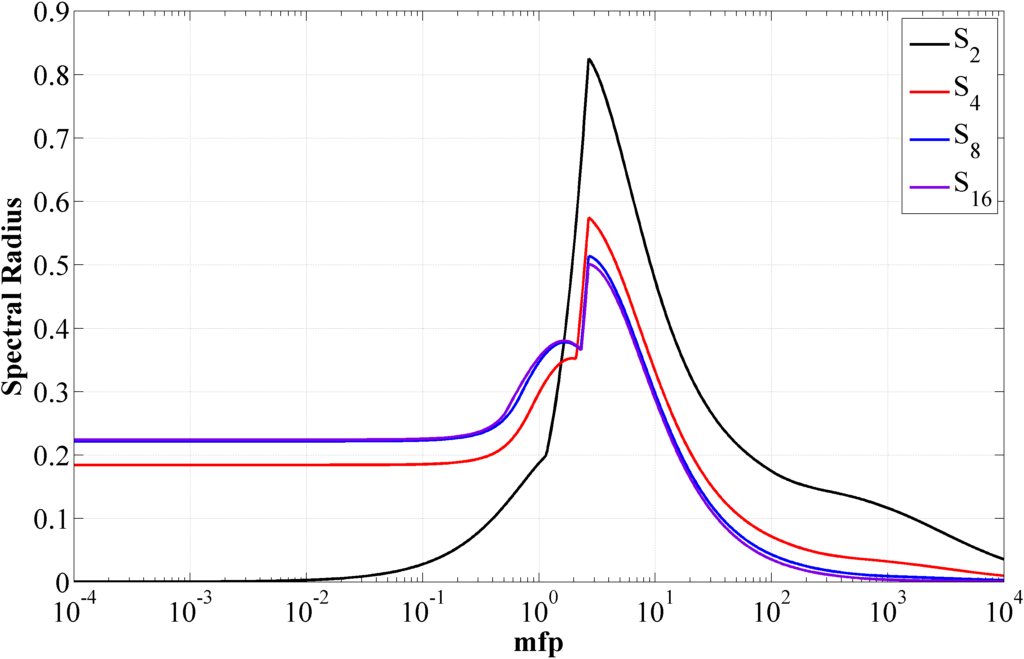
\includegraphics[width=\textwidth]{figures/appendices/DSA_1D_SI_MIP_C=1.png}
\caption{Spectral radius for the 1D MIP form using $c=1$.}
\label{fig::1D_MIP_c=1}
\end{figure}

\begin{figure}
\centering
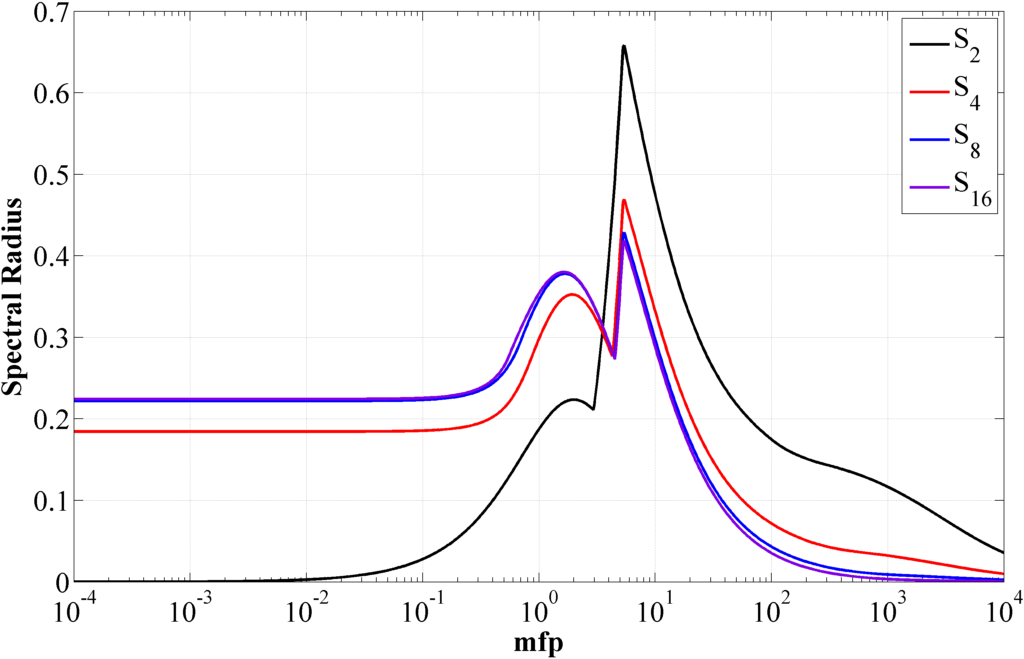
\includegraphics[width=\textwidth]{figures/appendices/DSA_1D_SI_MIP_C=2.png}
\caption{Spectral radius for the 1D MIP form using $c=2$.}
\label{fig::1D_MIP_c=2}
\end{figure}

\begin{figure}
\centering
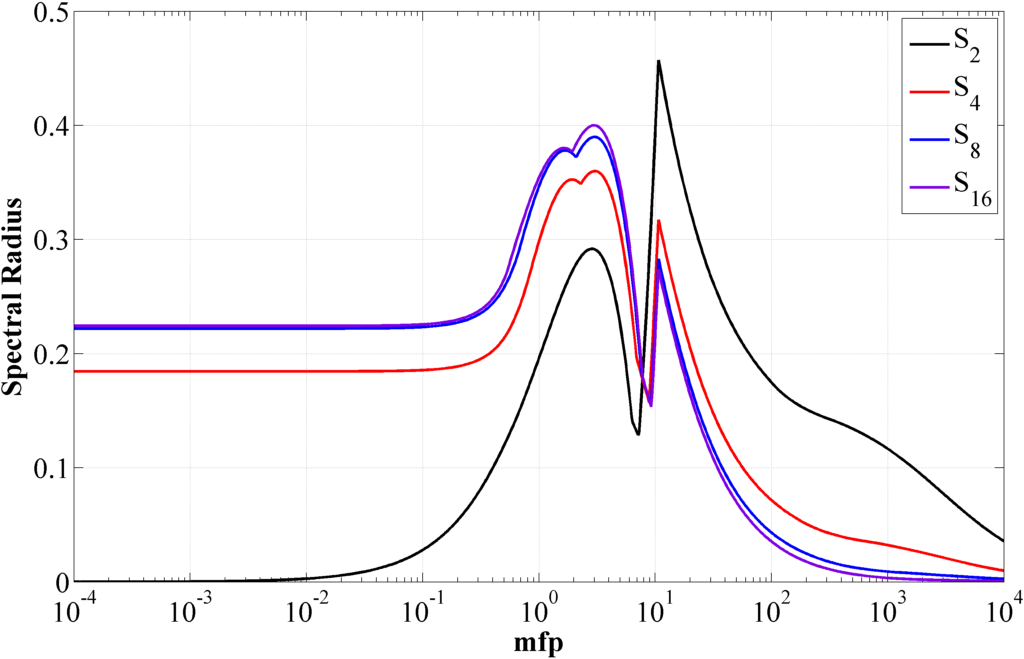
\includegraphics[width=\textwidth]{figures/appendices/DSA_1D_SI_MIP_C=4.png}
\caption{Spectral radius for the 1D MIP form using $c=4$.}
\label{fig::1D_MIP_c=4}
\end{figure}

\begin{figure}
\centering
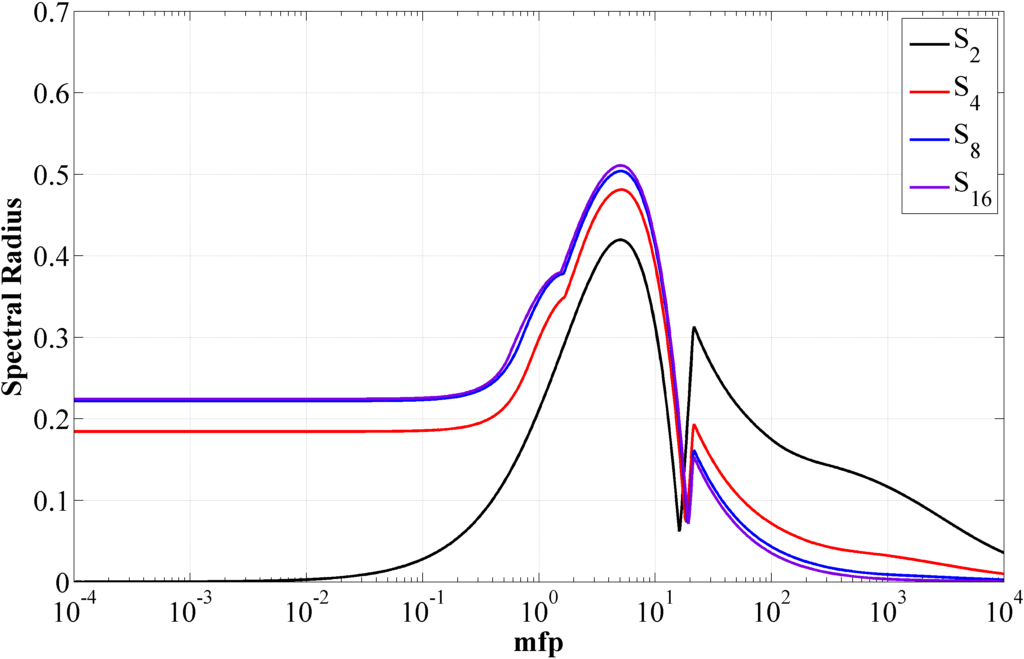
\includegraphics[width=\textwidth]{figures/appendices/DSA_1D_SI_MIP_C=8.png}
\caption{Spectral radius for the 1D MIP form using $c=8$.}
\label{fig::1D_MIP_c=8}
\end{figure}

\begin{figure}
\centering
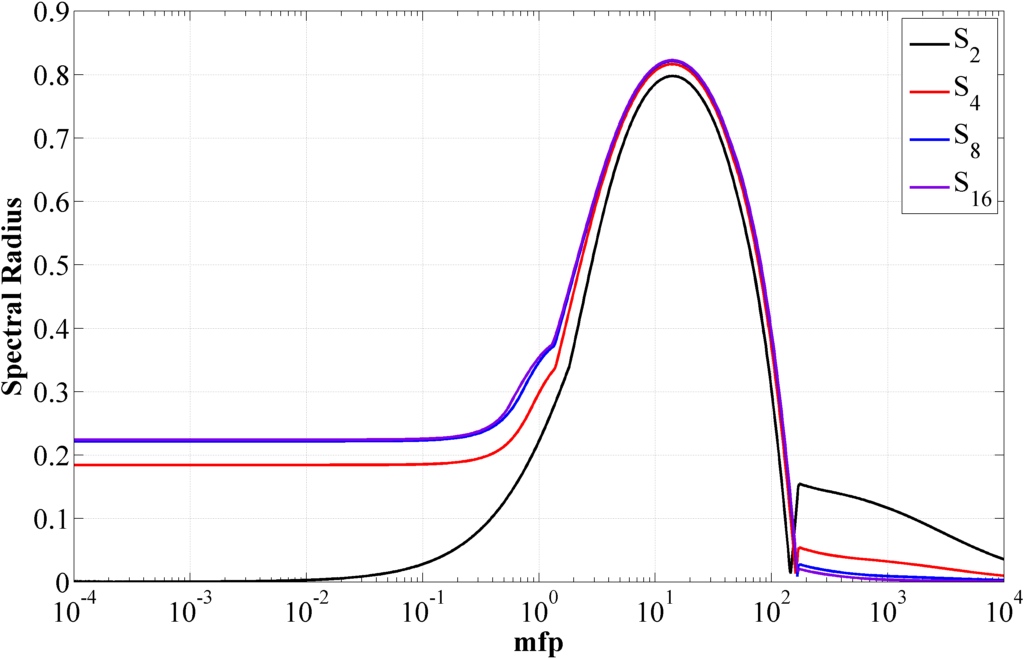
\includegraphics[width=\textwidth]{figures/appendices/DSA_1D_SI_MIP_C=64.png}
\caption{Spectral radius for the 1D MIP form using $c=64$.}
\label{fig::1D_MIP_c=64}
\end{figure}
\iffalse
\begin{figure}
\centering
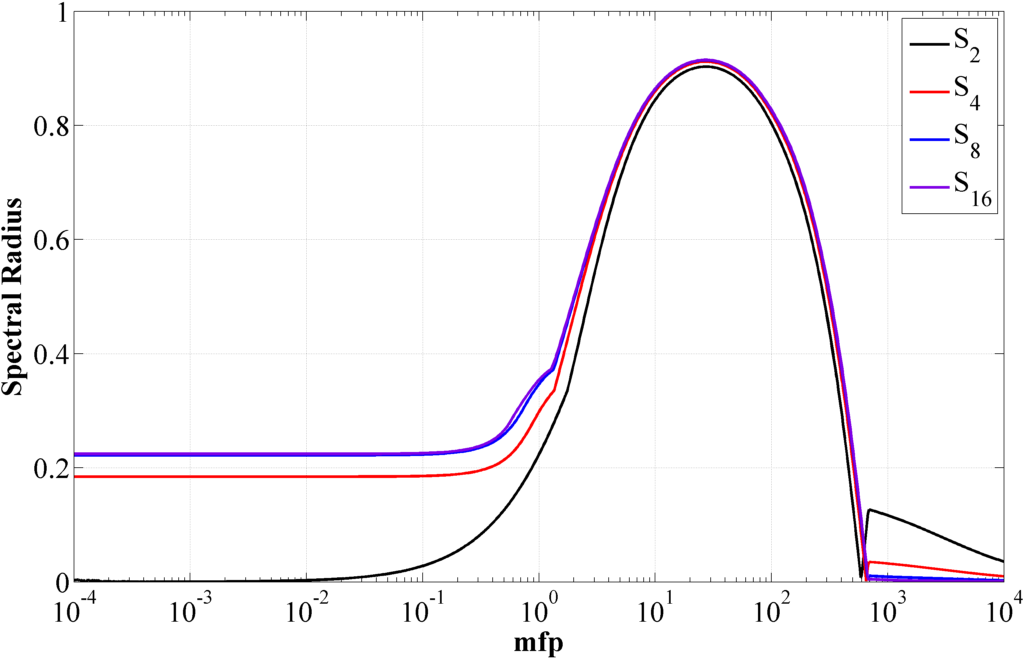
\includegraphics[width=\textwidth]{figures/appendices/DSA_1D_SI_MIP_C=256.png}
\caption{Spectral radius for the 1D MIP form using $c=256$.}
\label{fig::1D_MIP_c=256}
\end{figure}
\fi
% End: IP and MIP 1D Fourier Plots
%%%%%%%%%%%%%%%%%%%%%%%%%%%%%%%%%%%%%%%%%%%%%%%%%%%%%%

%%%%%%%%%%%%%%%%%%%%%%%%%%%%%%%%%%%%%%%%%%%%%%%%%%%
%%%%%%%%%%%%%%%%%%%%%%%%%%%%%%%%%%%%%%%%%%%%%%%%%%%
%%%   Section - M4S and MIP Comparison
%%%%%%%%%%%%%%%%%%%%%%%%%%%%%%%%%%%%%%%%%%%%%%%%%%%
%%%%%%%%%%%%%%%%%%%%%%%%%%%%%%%%%%%%%%%%%%%%%%%%%%%
\newpage
\section{Comparison between Modified Interior Penalty and Modified Four-Step DSA Schemes}
\label{sec::App_DSA_M4S}

In this work, our low-order diffusion operator was the discontinuous DFEM MIP form. Another common, fully-discontinuous form of the diffusion equation for use as a DSA scheme is the Modified Four-Step (M4S) method \cite{ref::dsa_DFEM_adams_martin}. It is a partially-consistent DSA scheme that can be derived in two-separate ways to yield the same functional form. One method is to take the analytic transport equation, expand the angular flux moments, take the moments to form the analytic diffusion equation, and then spatially discretize to form the spatially discretized diffusion equation. Conversely, the derivation can be performed by spatially discretizing the analytic transport equation, expanding the angular flux moments, and taking the moments to form the spatially discretized diffusion equation. Using either of these methods, 


With the notation that we used for the SIP and MIP forms in Chapter \ref{sec::DSA}, we can write the M4S diffusion form as 

\begin{equation}
a^{M4S}( b, \delta \Phi) = b^{M4S}(b),
\label{eq::M4S_weak_form}
\end{equation}

\noindent with the following bilinear matrix,

\begin{equation}
\label{eq::M4S_bilinear_form}
\begin{aligned}
a^{M4S}(b, \delta \Phi)  = \Big(  D \vec{\nabla} b , \vec{\nabla} \delta \Phi  \Big)_{\mathcal{D}} + \Big(  \sigma b , \delta \Phi  \Big)_{\mathcal{D}}    \\
+ \frac{1}{4}  \Big< [\![   b ]\!] , [\![  \delta \Phi ]\!]\Big>_{E_h^i} + \Big<  [\![  b ]\!] , \{\!\{  D \partial_n \delta \Phi \}\!\}\Big>_{E_h^i}   \\
+ \frac{1}{4} \Big<   b , \delta  \Phi \Big>_{\partial \mathcal{D}^d} - \frac{1}{2} \Big<  b ,  D \partial_n \delta \Phi \Big>_{\partial \mathcal{D}^d} 
\end{aligned} ,
\end{equation}

\noindent and with the following linear right-hand-side,

\begin{equation}
\label{eq::M4S_linear_form}
b^{M4S} (b) = \Big(  b, Q  \Big)_{\mathcal{D}}   .
\end{equation}

\noindent We note that we have employed only incident boundary conditions, $\partial \mathcal{D}^d$. From Eq. (\ref{eq::M4S_bilinear_form}), we can see that there are similarities between the M4S and MIP bilinear forms. In particular, we can arrive at the M4S form by always setting the MIP penalty coefficient to be 1/4 and omitting the $\Big< \{\!\{  D \partial_n b \}\!\} , [\![ \delta \Phi ]\!]\Big>_{E_h^i}$ and $\frac{1}{2} \Big<   D \partial_n b , \delta \Phi \Big>_{\partial \mathcal{D}^d}$ terms. 

We now provide a pair of results for the M4S form. First, we give a comparison between the theoretical Fourier Analysis and numerical spectral radii results on unit square mesh cells using the linear PWL basis functions in Figure \ref{fig::App_DSA_2D_M4S_Fourier_NSR}. Then, we provide the Fourier wave number distributions of the PWL basis functions on the unit square in Figures \ref{fig::App_DSA_M4S_LS2}, \ref{fig::App_DSA_M4S_LS4}, \ref{fig::App_DSA_M4S_LS8}, and \ref{fig::App_DSA_M4S_LS16} for the $S_2$, $S_4$, $S_8$, and $S_16$ level-symmetric quadrature, respectively.


% BEGIN M4S PLOTS
\begin{figure}
\centering
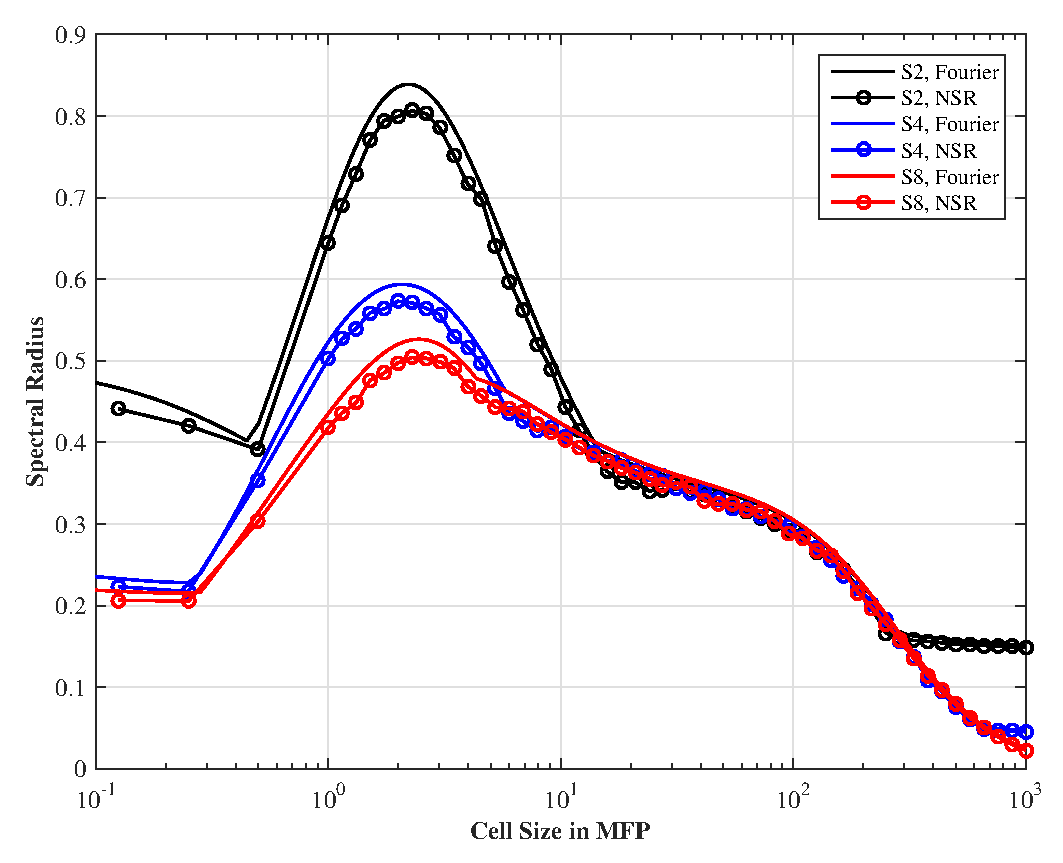
\includegraphics[width=0.85\textwidth]{figures/appendices/SI_M4S_2D_wNSR.eps}
\caption{Comparison between the numerical spectral radii and the theoretical Fourier Analysis spectral radii for the M4S scheme on the unit square.}
\label{fig::App_DSA_2D_M4S_Fourier_NSR}
\end{figure}

\begin{figure}
\centering
	{
	\begin{subfigure}[b]{0.485\textwidth}
		\centering
		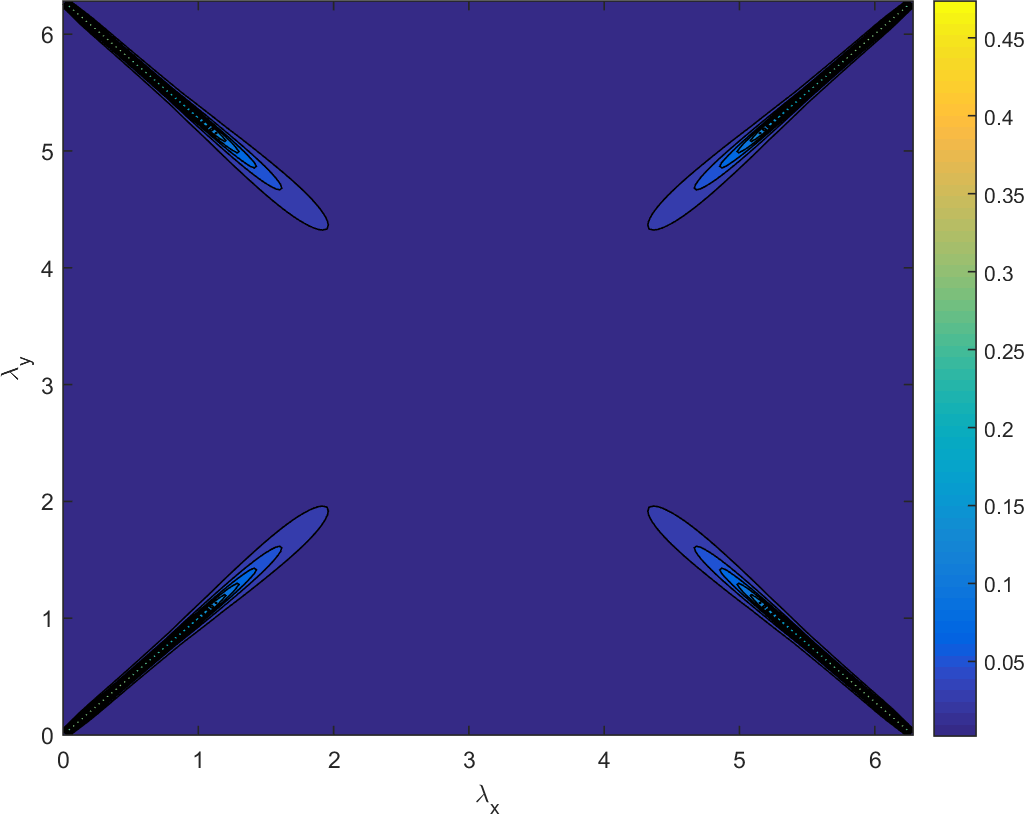
\includegraphics[width=0.975\textwidth]{figures/appendices/SI_M4S_UPWLD1_LS2_x=1e-2_dydx=1_contour.png}
		\caption{$10^{-2}$ mfp}
	\end{subfigure}
	\hfill
	\begin{subfigure}[b]{0.485\textwidth}
		\centering
		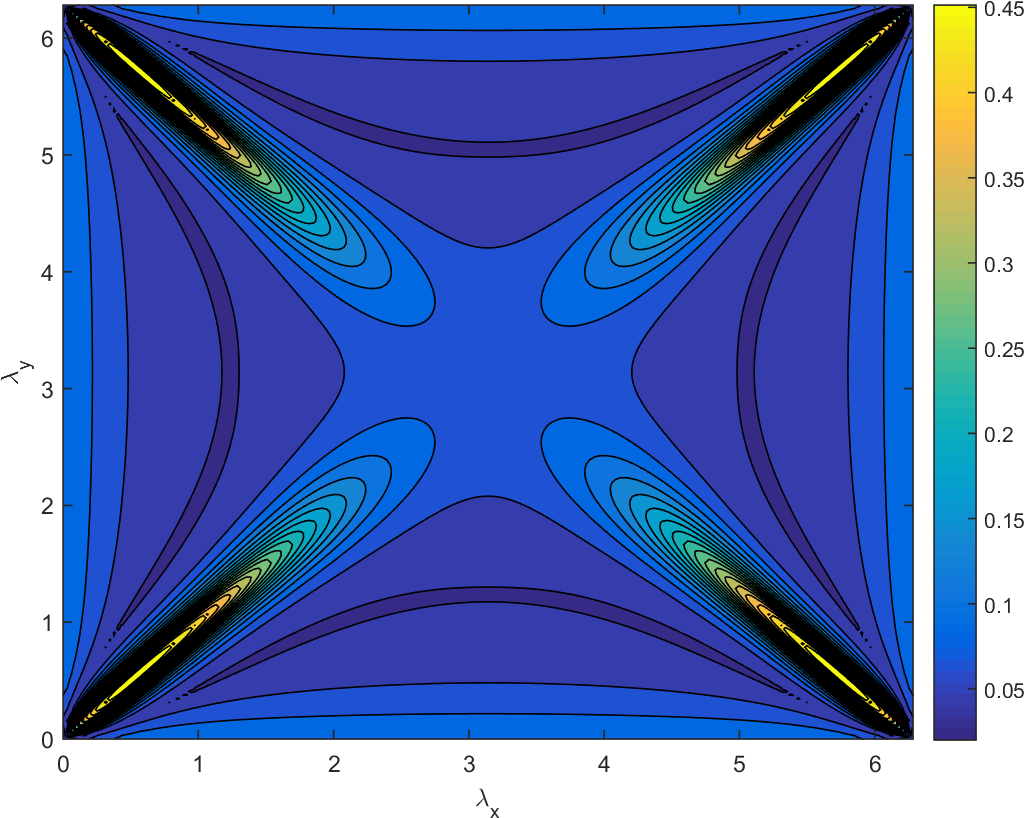
\includegraphics[width=0.975\textwidth]{figures/appendices/SI_M4S_UPWLD1_LS2_x=1e-1_dydx=1_contour.png}
		\caption{$10^{-1}$ mfp}
	\end{subfigure}
	}
	\vspace{0.5cm}
	{
	\begin{subfigure}[b]{0.485\textwidth}
		\centering
		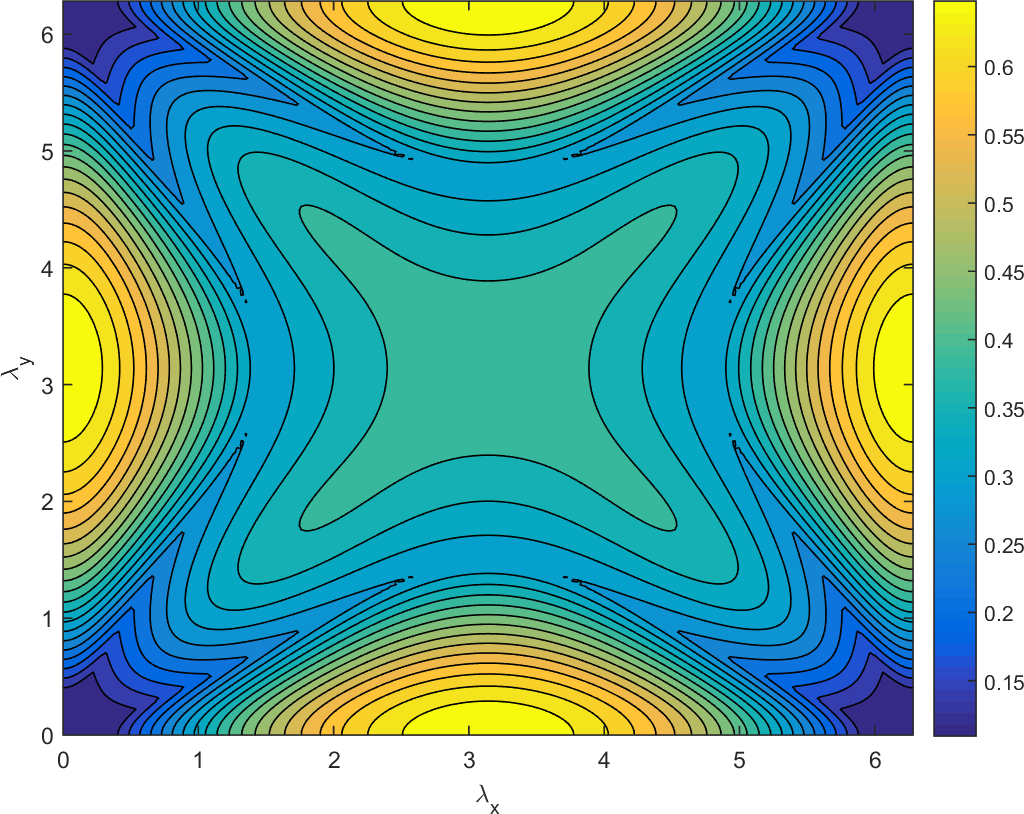
\includegraphics[width=0.975\textwidth]{figures/appendices/SI_M4S_UPWLD1_LS2_x=1_dydx=1_contour.png}
		\caption{$10^{0}$ mfp}
	\end{subfigure}
	\hfill
	\begin{subfigure}[b]{0.485\textwidth}
		\centering
		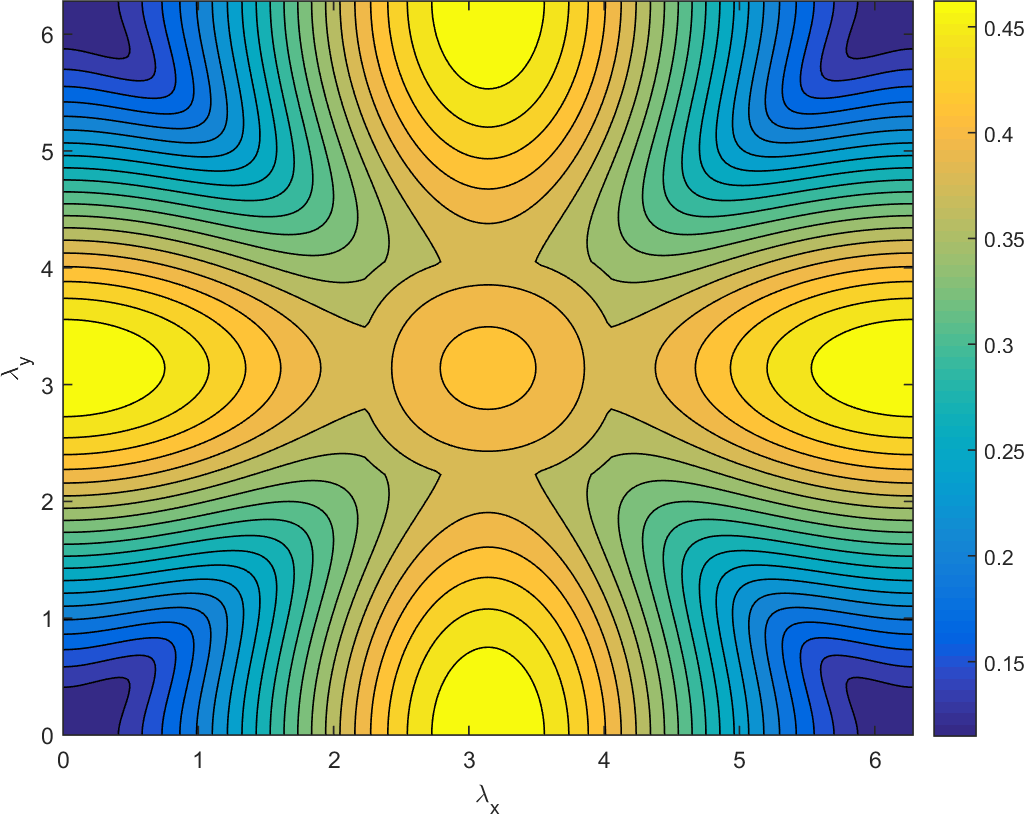
\includegraphics[width=0.975\textwidth]{figures/appendices/SI_M4S_UPWLD1_LS2_x=10_dydx=1_contour.png}
		\caption{$10^{1}$ mfp}
	\end{subfigure}
	}
	\vspace{0.5cm}
	{
	\begin{subfigure}[b]{0.485\textwidth}
		\centering
		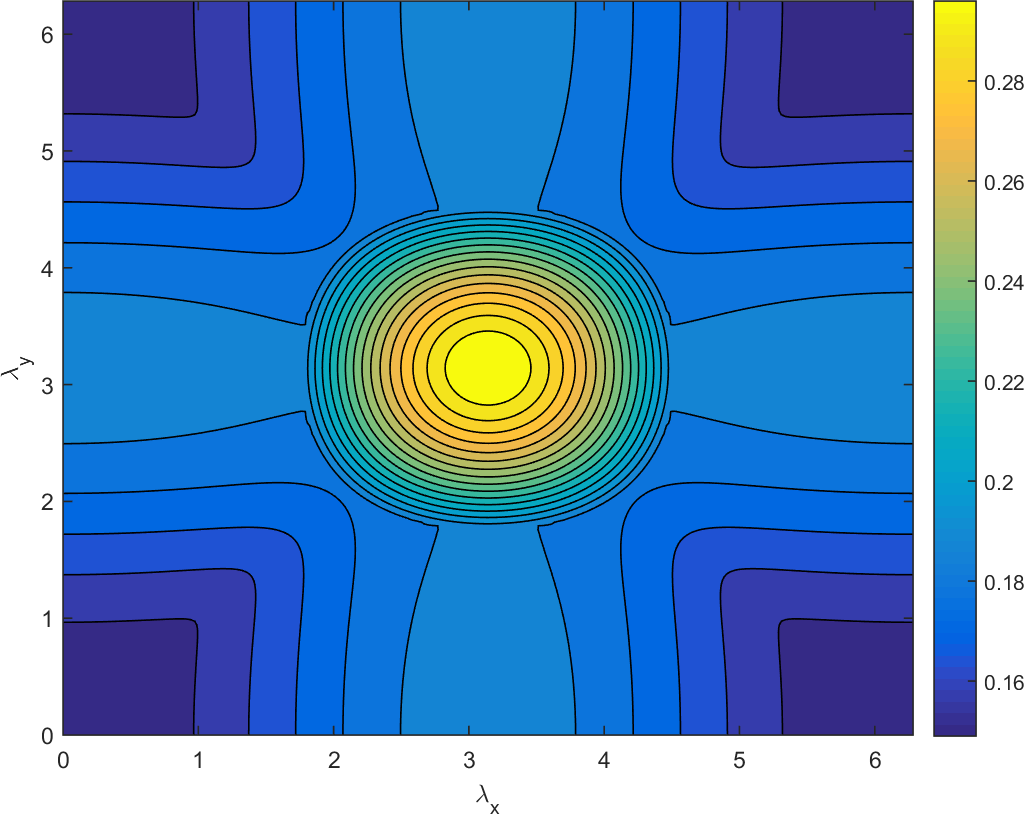
\includegraphics[width=0.975\textwidth]{figures/appendices/SI_M4S_UPWLD1_LS2_x=100_dydx=1_contour.png}
		\caption{$10^{2}$ mfp}
	\end{subfigure}
	\hfill
	\begin{subfigure}[b]{0.485\textwidth}
		\centering
		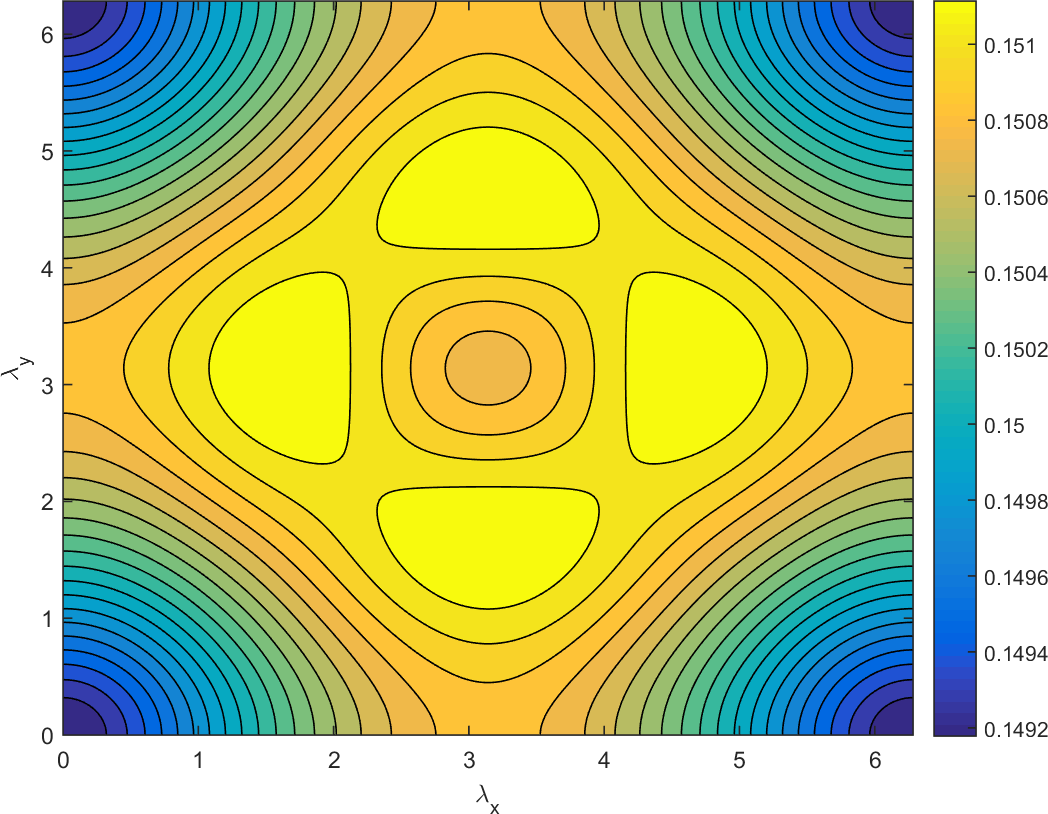
\includegraphics[width=0.975\textwidth]{figures/appendices/SI_M4S_UPWLD1_LS2_x=1000_dydx=1_contour.png}
		\caption{$10^{3}$ mfp}
	\end{subfigure}
	}
\caption{Fourier wave number distribution for different mesh optical thicknesses of a single 2D square cell with PWL basis functions and $LS_{2}$ quadrature.}
\label{fig::App_DSA_M4S_LS2}
\end{figure}

\begin{figure}
\centering
	{
	\begin{subfigure}[b]{0.485\textwidth}
		\centering
		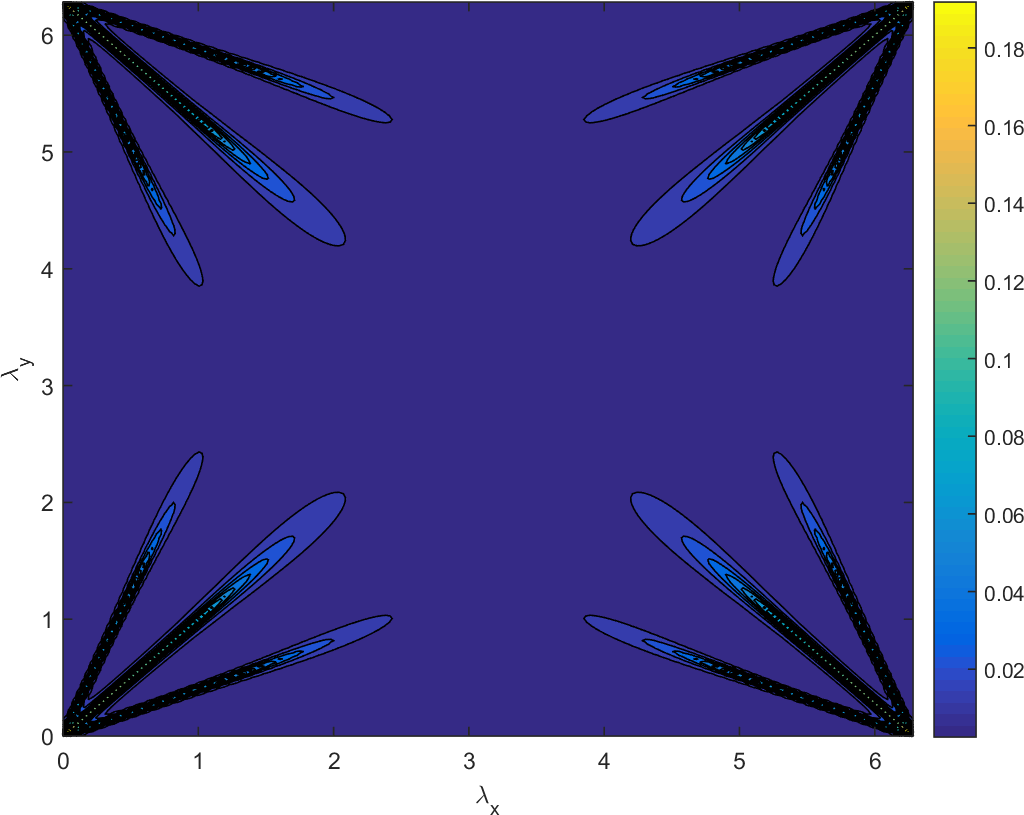
\includegraphics[width=0.975\textwidth]{figures/appendices/SI_M4S_UPWLD1_LS4_x=1e-2_dydx=1_contour.png}
		\caption{$10^{-2}$ mfp}
	\end{subfigure}
	\hfill
	\begin{subfigure}[b]{0.485\textwidth}
		\centering
		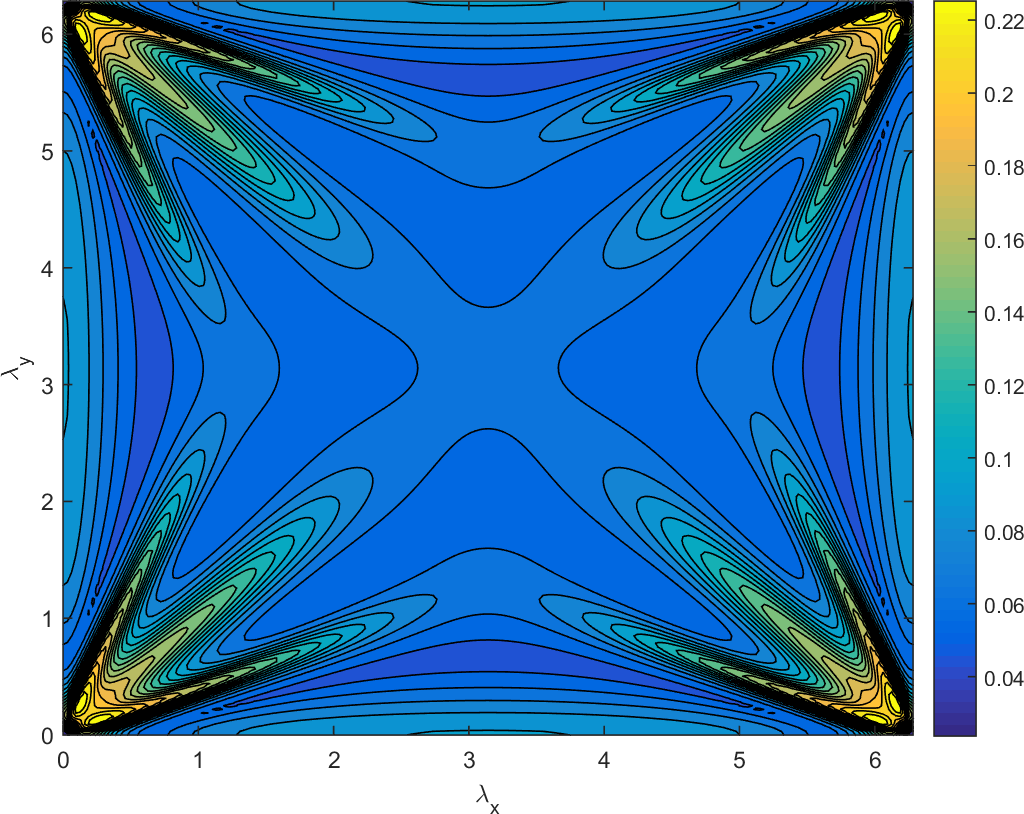
\includegraphics[width=0.975\textwidth]{figures/appendices/SI_M4S_UPWLD1_LS4_x=1e-1_dydx=1_contour.png}
		\caption{$10^{-1}$ mfp}
	\end{subfigure}
	}
	\vspace{0.5cm}
	{
	\begin{subfigure}[b]{0.485\textwidth}
		\centering
		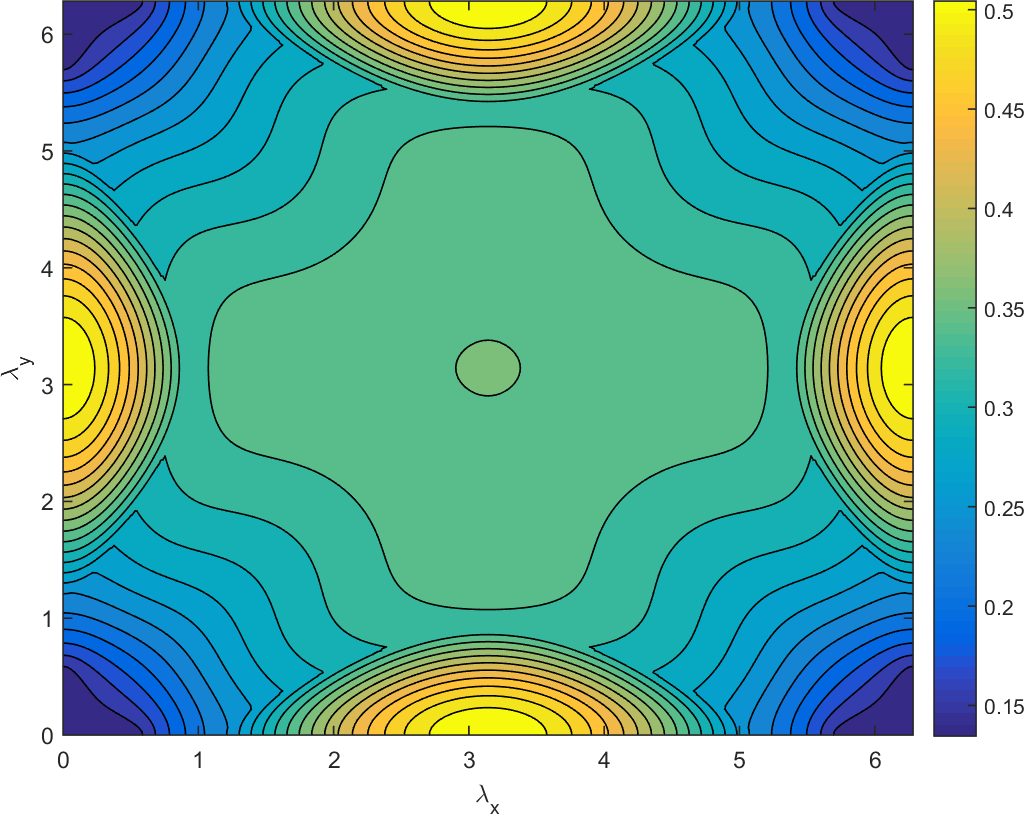
\includegraphics[width=0.975\textwidth]{figures/appendices/SI_M4S_UPWLD1_LS4_x=1_dydx=1_contour.png}
		\caption{$10^{0}$ mfp}
	\end{subfigure}
	\hfill
	\begin{subfigure}[b]{0.485\textwidth}
		\centering
		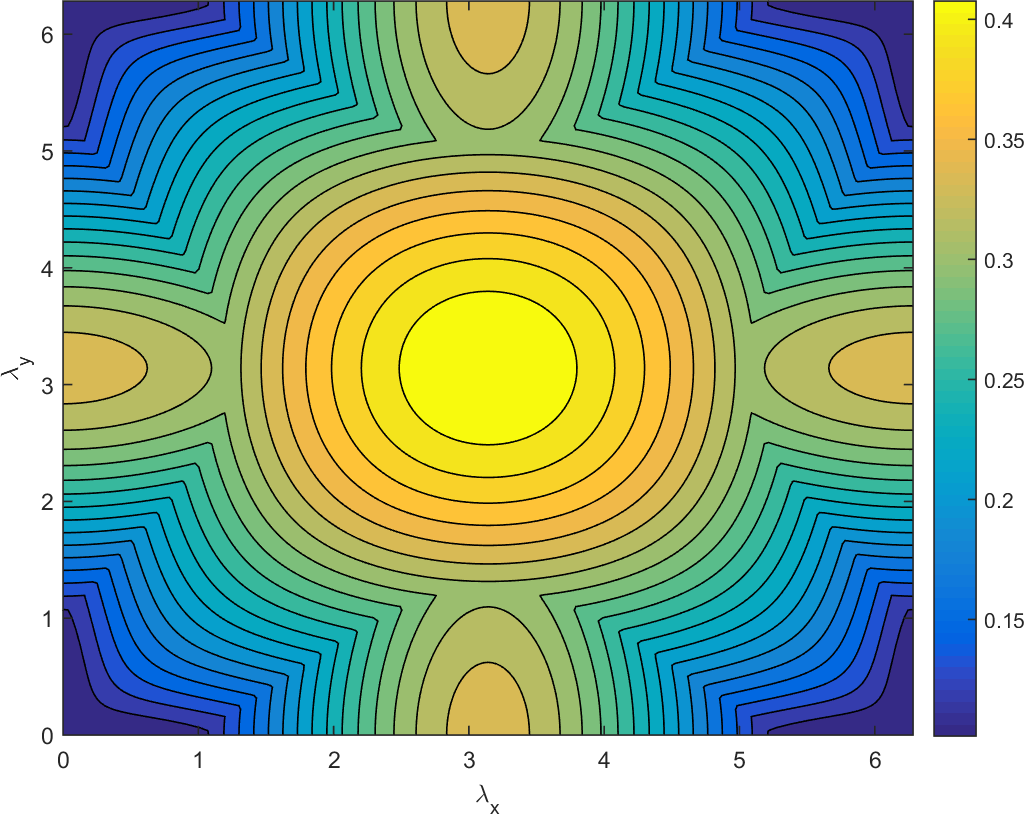
\includegraphics[width=0.975\textwidth]{figures/appendices/SI_M4S_UPWLD1_LS4_x=10_dydx=1_contour.png}
		\caption{$10^{1}$ mfp}
	\end{subfigure}
	}
	\vspace{0.5cm}
	{
	\begin{subfigure}[b]{0.485\textwidth}
		\centering
		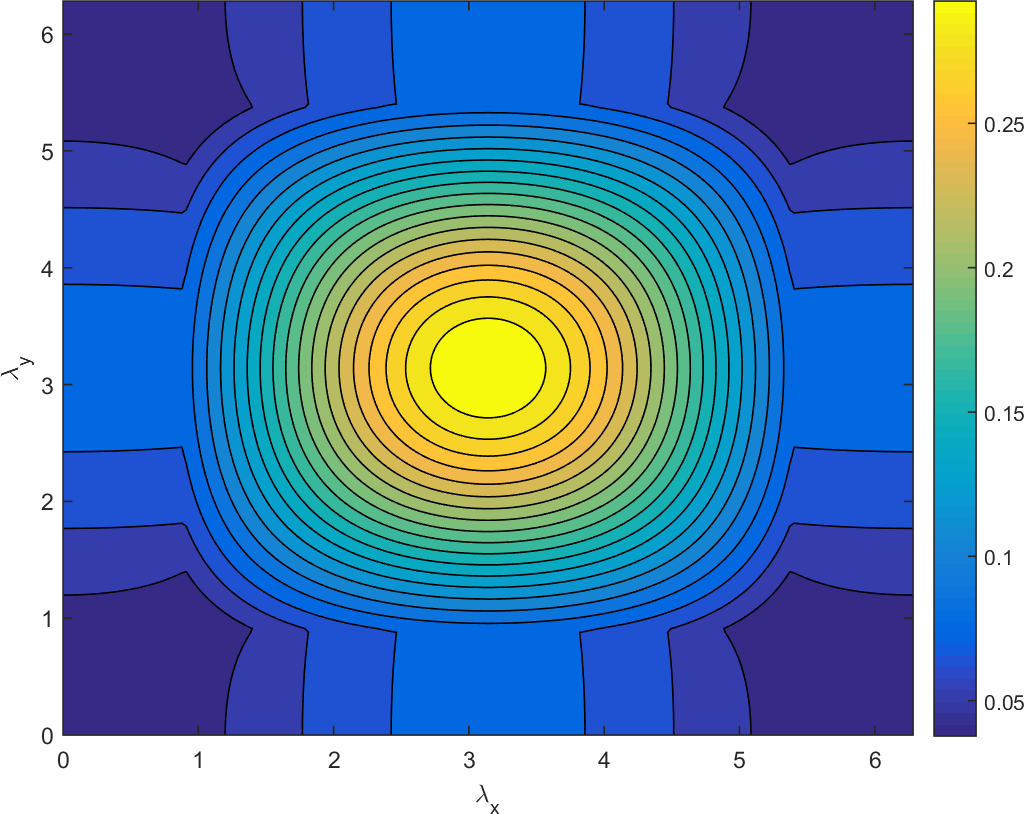
\includegraphics[width=0.975\textwidth]{figures/appendices/SI_M4S_UPWLD1_LS4_x=100_dydx=1_contour.png}
		\caption{$10^{2}$ mfp}
	\end{subfigure}
	\hfill
	\begin{subfigure}[b]{0.485\textwidth}
		\centering
		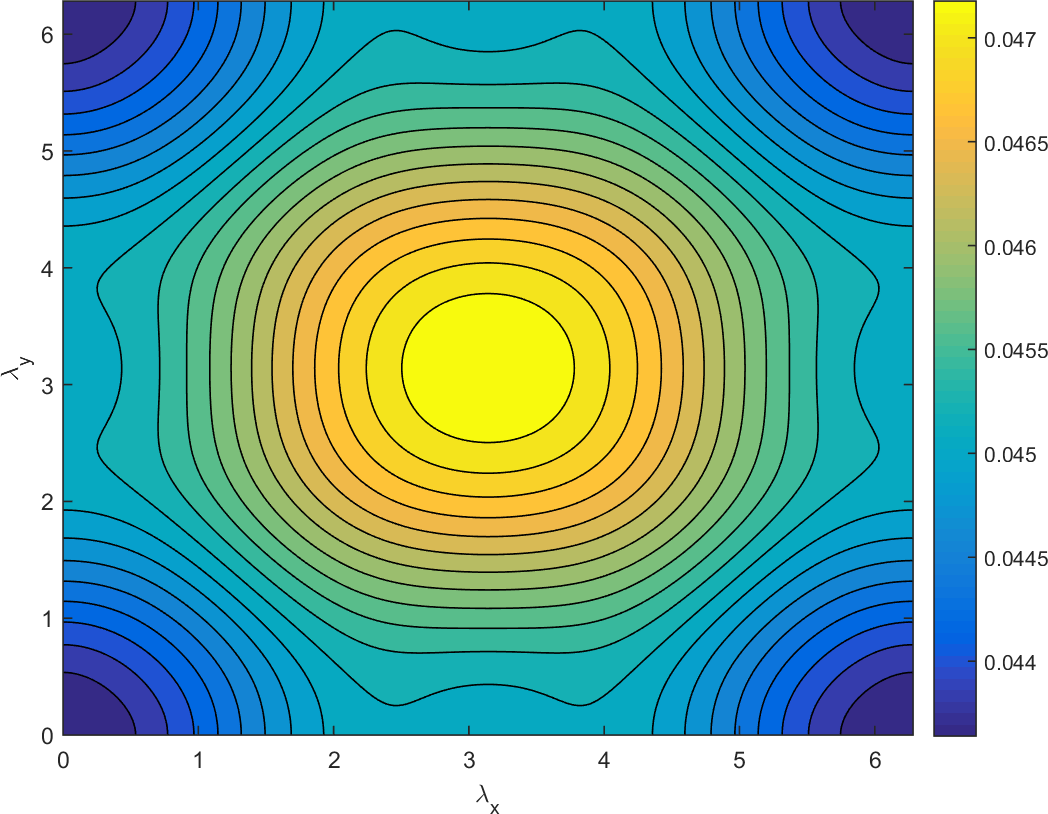
\includegraphics[width=0.975\textwidth]{figures/appendices/SI_M4S_UPWLD1_LS4_x=1000_dydx=1_contour.png}
		\caption{$10^{3}$ mfp}
	\end{subfigure}
	}
\caption{Fourier wave number distribution for different mesh optical thicknesses of a single 2D square cell with PWL basis functions and $LS_{4}$ quadrature.}
\label{fig::App_DSA_M4S_LS4}
\end{figure}

\begin{figure}
\centering
	{
	\begin{subfigure}[b]{0.485\textwidth}
		\centering
		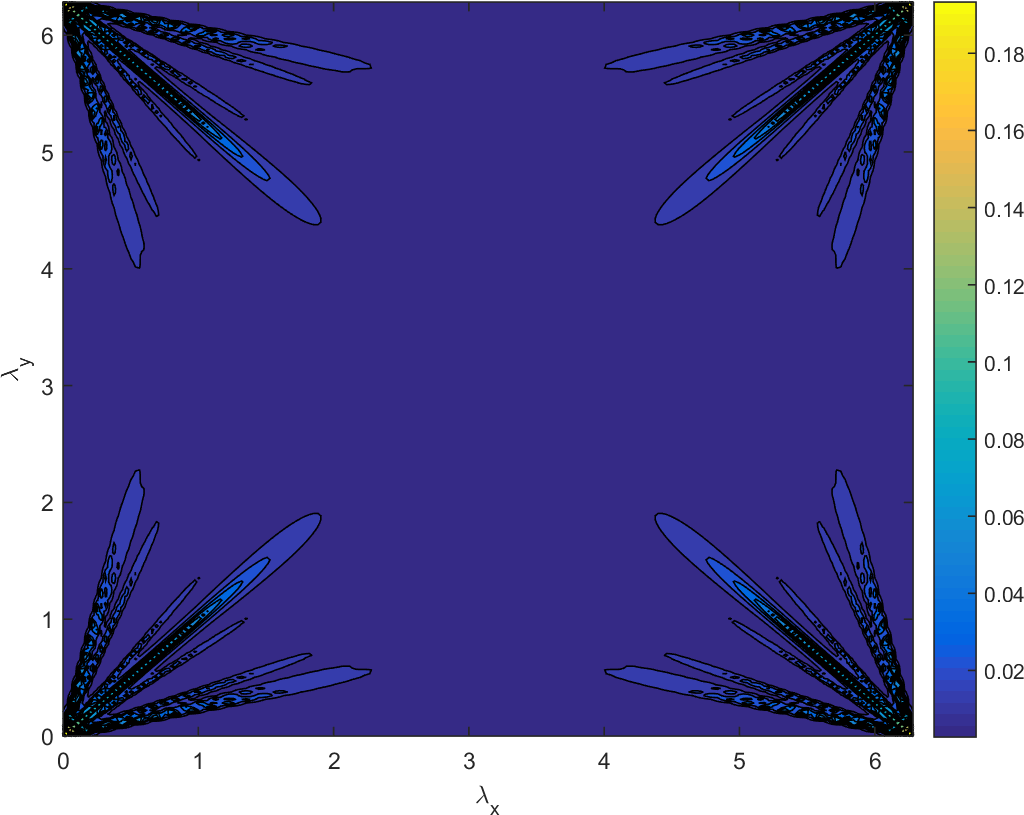
\includegraphics[width=0.975\textwidth]{figures/appendices/SI_M4S_UPWLD1_LS8_x=1e-2_dydx=1_contour.png}
		\caption{$10^{-2}$ mfp}
	\end{subfigure}
	\hfill
	\begin{subfigure}[b]{0.485\textwidth}
		\centering
		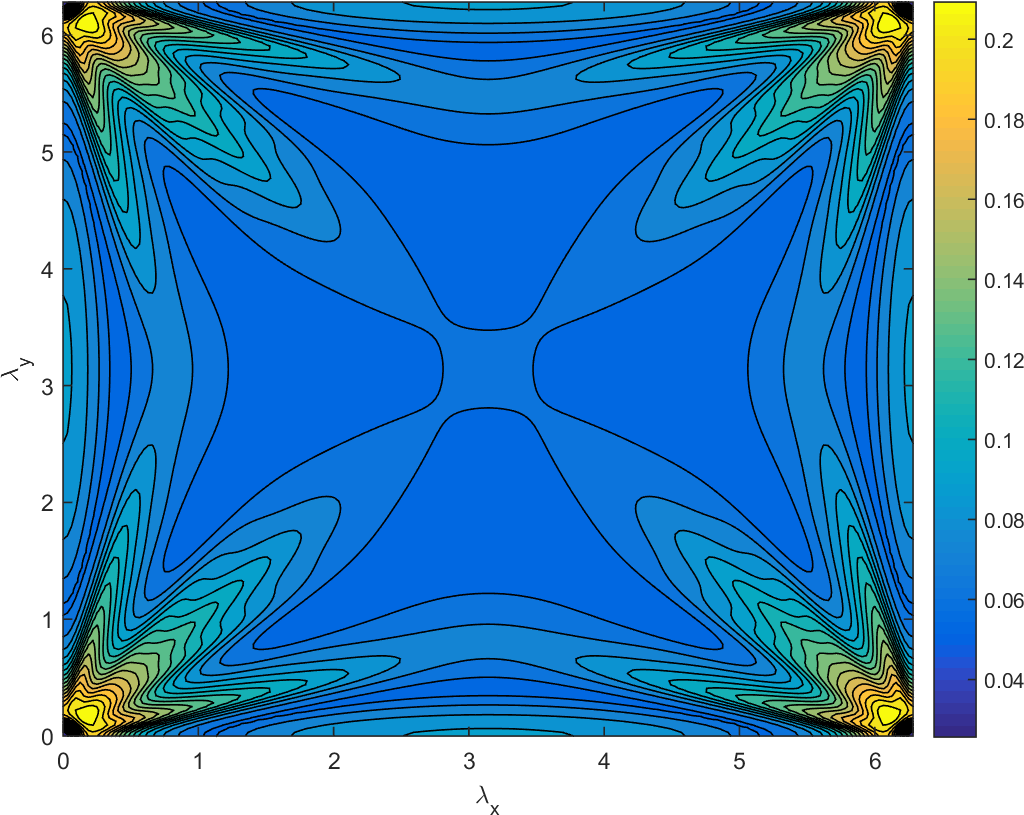
\includegraphics[width=0.975\textwidth]{figures/appendices/SI_M4S_UPWLD1_LS8_x=1e-1_dydx=1_contour.png}
		\caption{$10^{-1}$ mfp}
	\end{subfigure}
	}
	\vspace{0.5cm}
	{
	\begin{subfigure}[b]{0.485\textwidth}
		\centering
		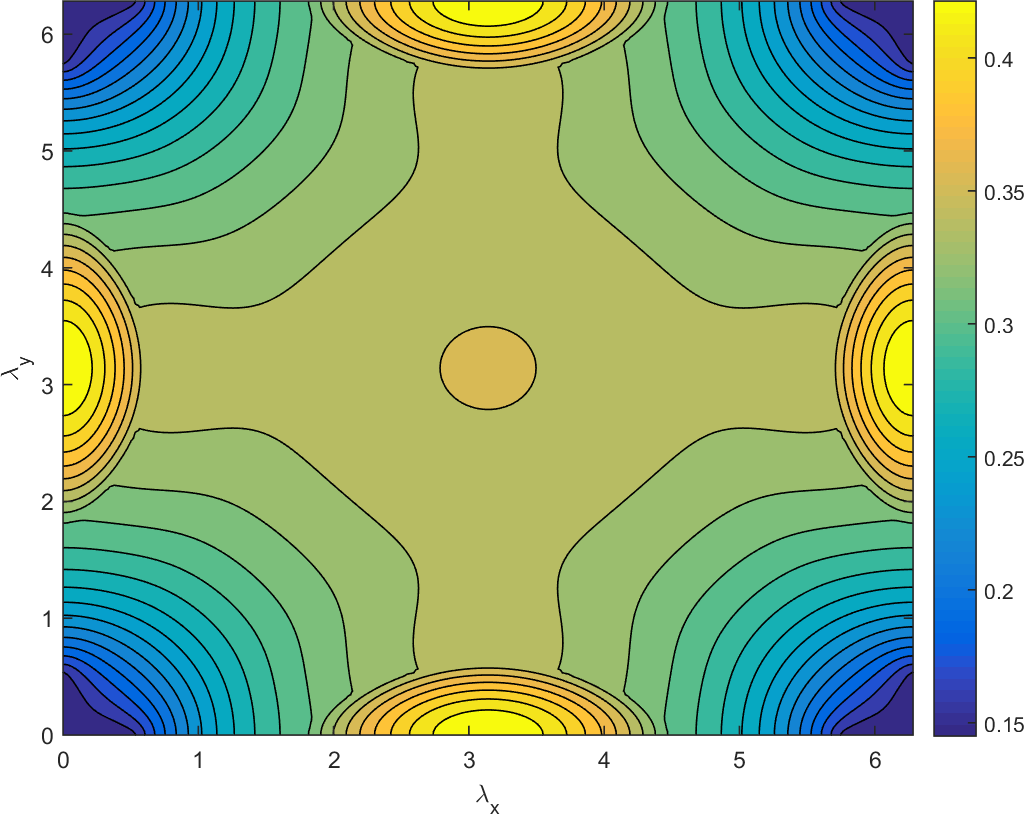
\includegraphics[width=0.975\textwidth]{figures/appendices/SI_M4S_UPWLD1_LS8_x=1_dydx=1_contour.png}
		\caption{$10^{0}$ mfp}
	\end{subfigure}
	\hfill
	\begin{subfigure}[b]{0.485\textwidth}
		\centering
		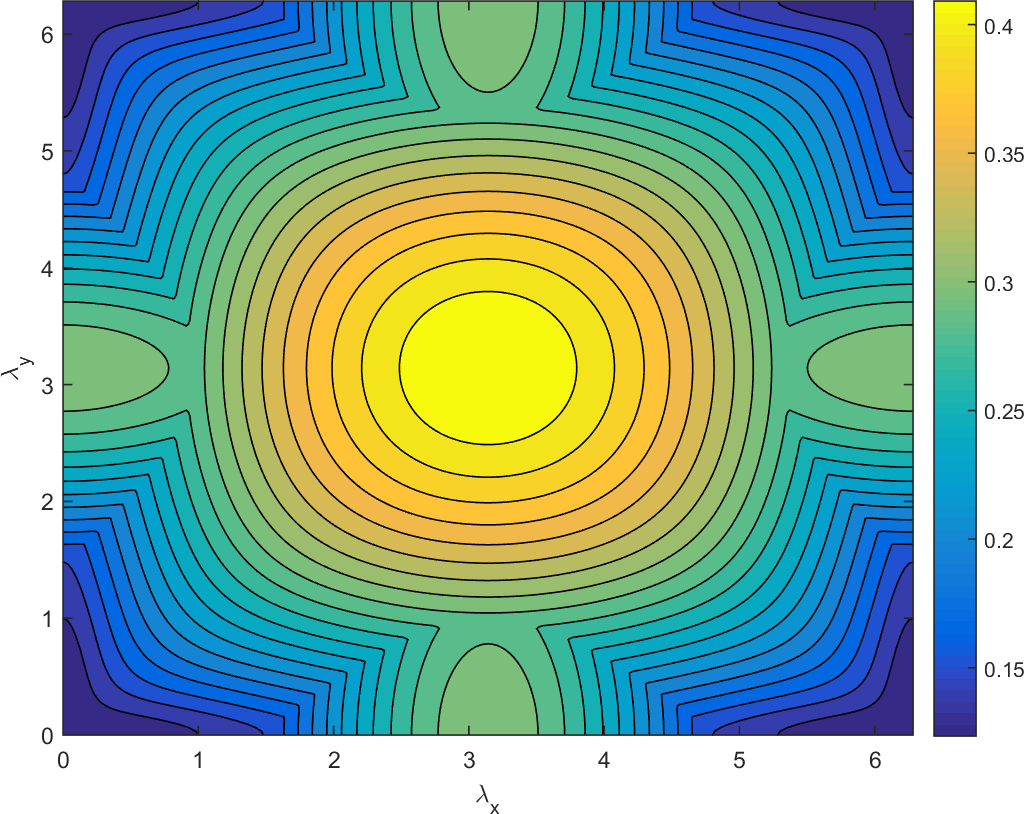
\includegraphics[width=0.975\textwidth]{figures/appendices/SI_M4S_UPWLD1_LS8_x=10_dydx=1_contour.png}
		\caption{$10^{1}$ mfp}
	\end{subfigure}
	}
	\vspace{0.5cm}
	{
	\begin{subfigure}[b]{0.485\textwidth}
		\centering
		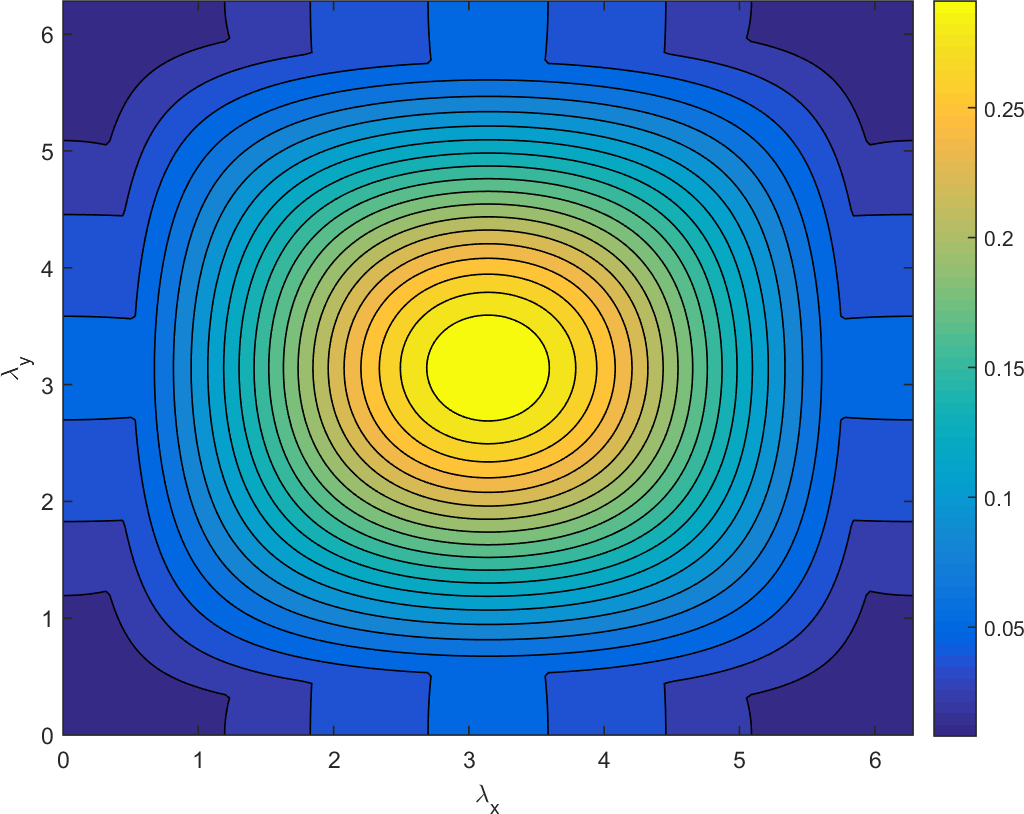
\includegraphics[width=0.975\textwidth]{figures/appendices/SI_M4S_UPWLD1_LS8_x=100_dydx=1_contour.png}
		\caption{$10^{2}$ mfp}
	\end{subfigure}
	\hfill
	\begin{subfigure}[b]{0.485\textwidth}
		\centering
		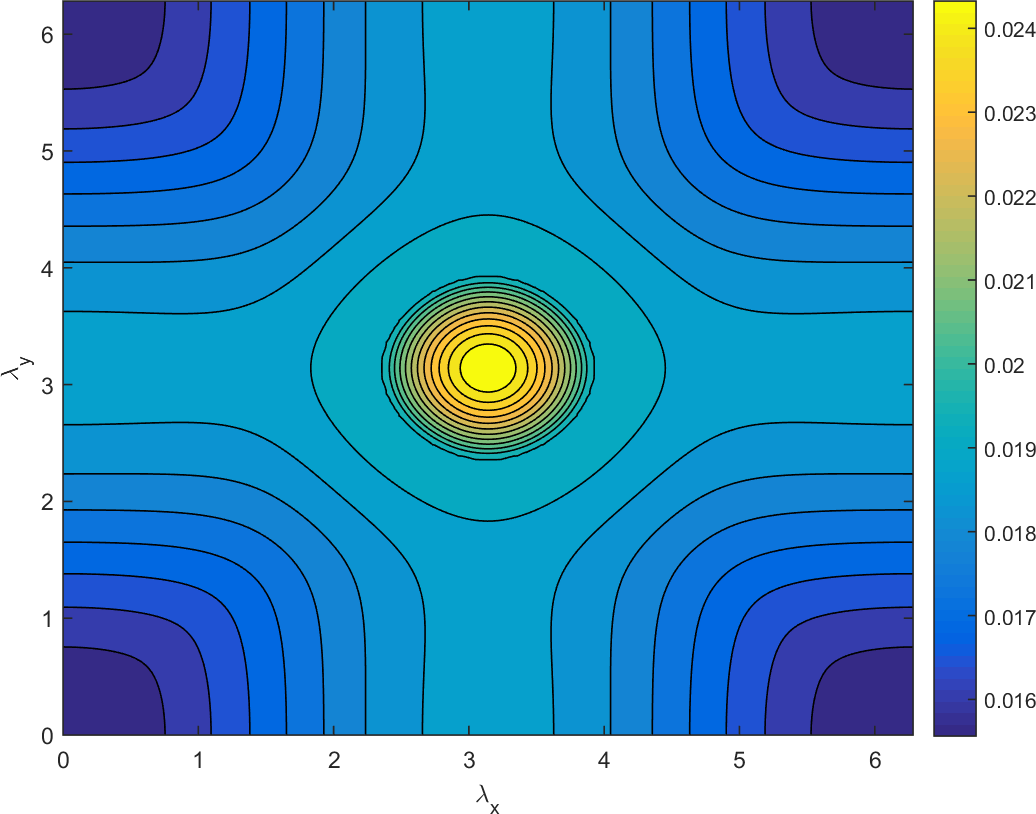
\includegraphics[width=0.975\textwidth]{figures/appendices/SI_M4S_UPWLD1_LS8_x=1000_dydx=1_contour.png}
		\caption{$10^{3}$ mfp}
	\end{subfigure}
	}
\caption{Fourier wave number distribution for different mesh optical thicknesses of a single 2D square cell with PWL basis functions and $LS_{8}$ quadrature.}
\label{fig::App_DSA_M4S_LS8}
\end{figure}

\begin{figure}
\centering
	{
	\begin{subfigure}[b]{0.485\textwidth}
		\centering
		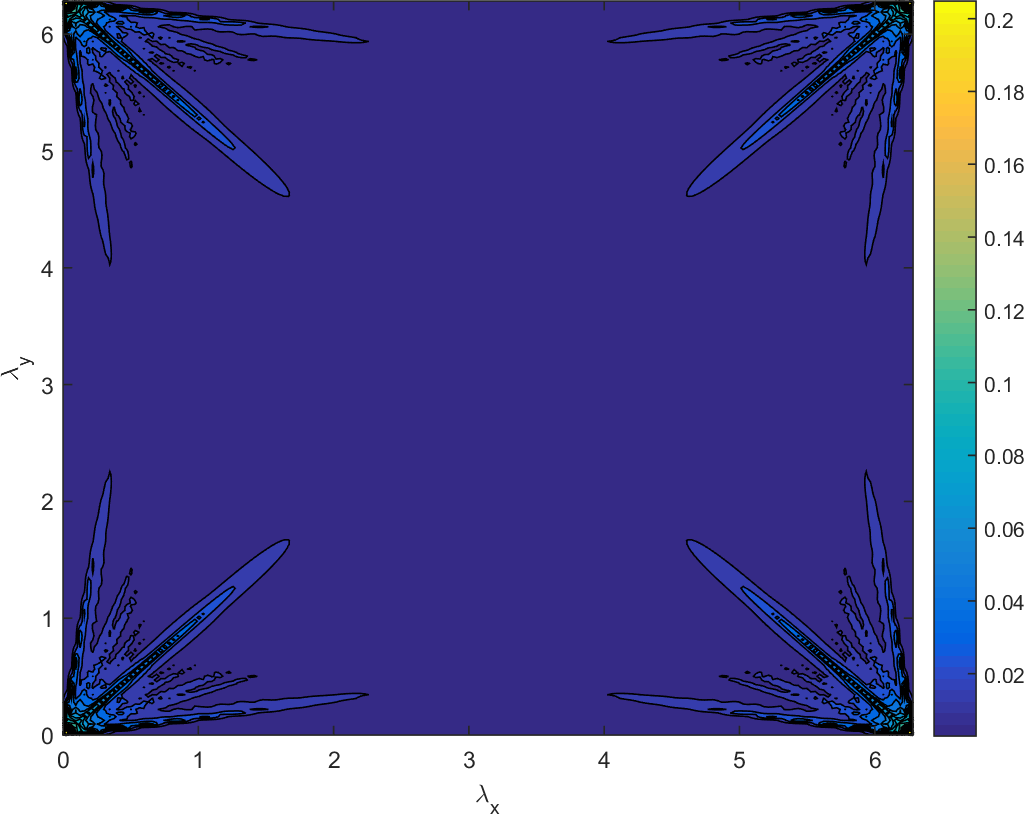
\includegraphics[width=0.975\textwidth]{figures/appendices/SI_M4S_UPWLD1_LS16_x=1e-2_dydx=1_contour.png}
		\caption{$10^{-2}$ mfp}
	\end{subfigure}
	\hfill
	\begin{subfigure}[b]{0.485\textwidth}
		\centering
		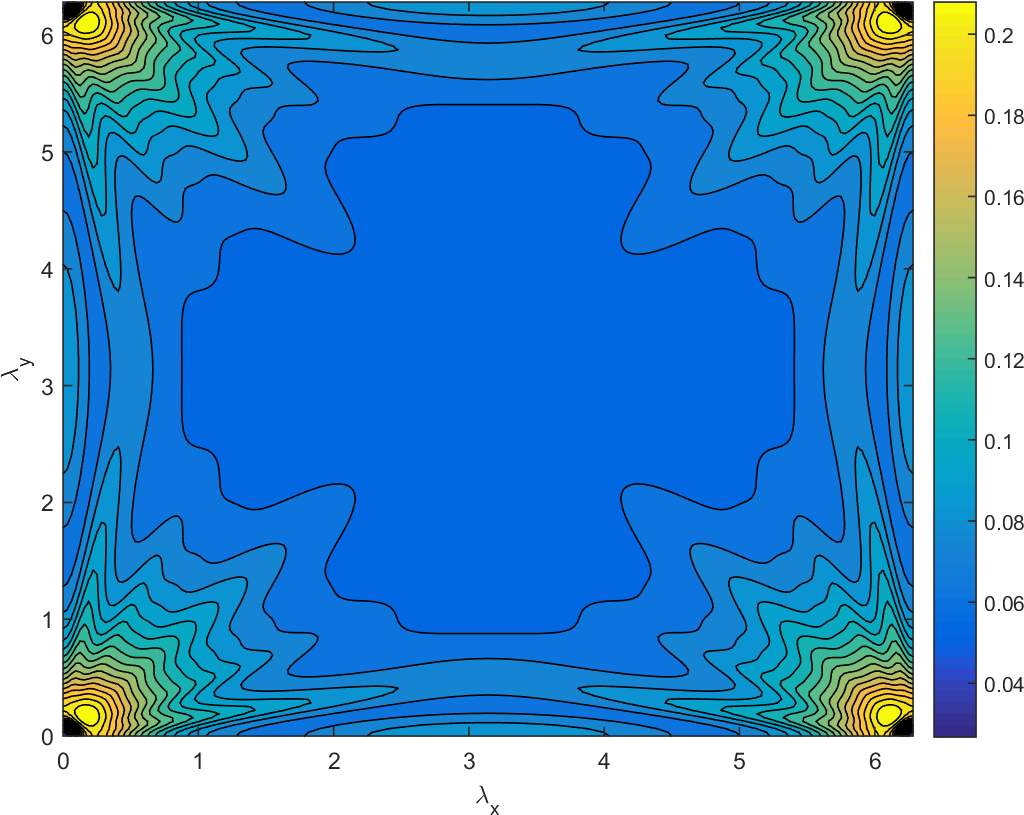
\includegraphics[width=0.975\textwidth]{figures/appendices/SI_M4S_UPWLD1_LS16_x=1e-1_dydx=1_contour.png}
		\caption{$10^{-1}$ mfp}
	\end{subfigure}
	}
	\vspace{0.5cm}
	{
	\begin{subfigure}[b]{0.485\textwidth}
		\centering
		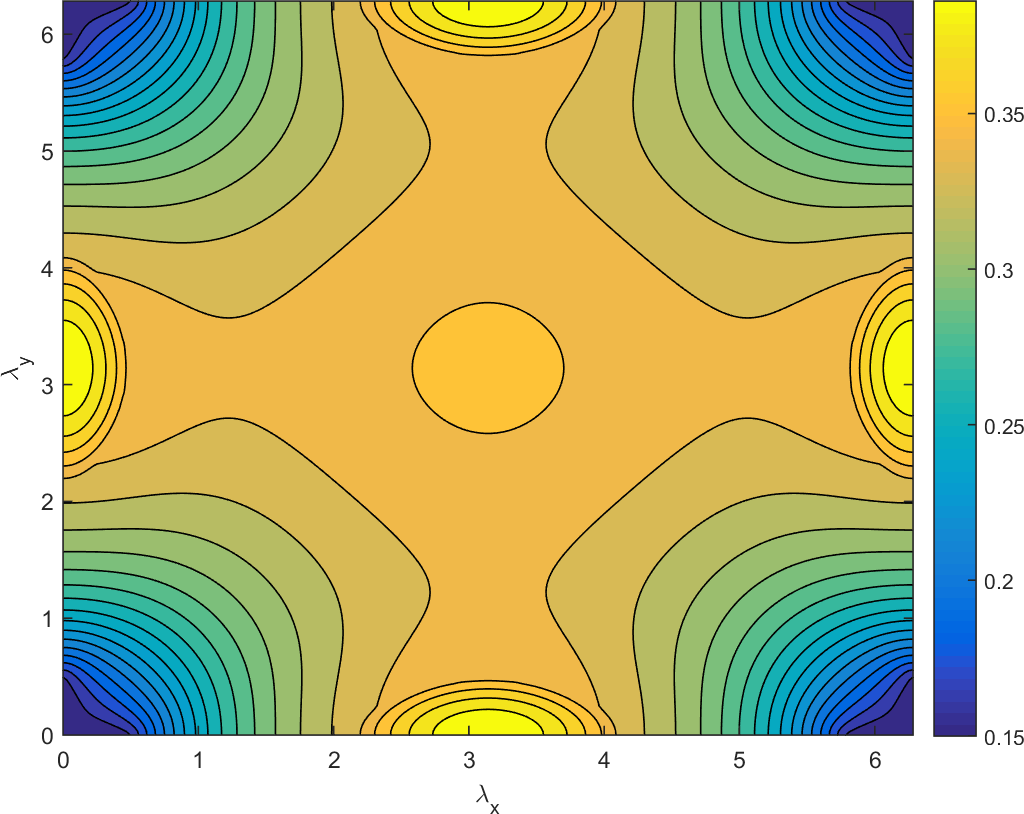
\includegraphics[width=0.975\textwidth]{figures/appendices/SI_M4S_UPWLD1_LS16_x=1_dydx=1_contour.png}
		\caption{$10^{0}$ mfp}
	\end{subfigure}
	\hfill
	\begin{subfigure}[b]{0.485\textwidth}
		\centering
		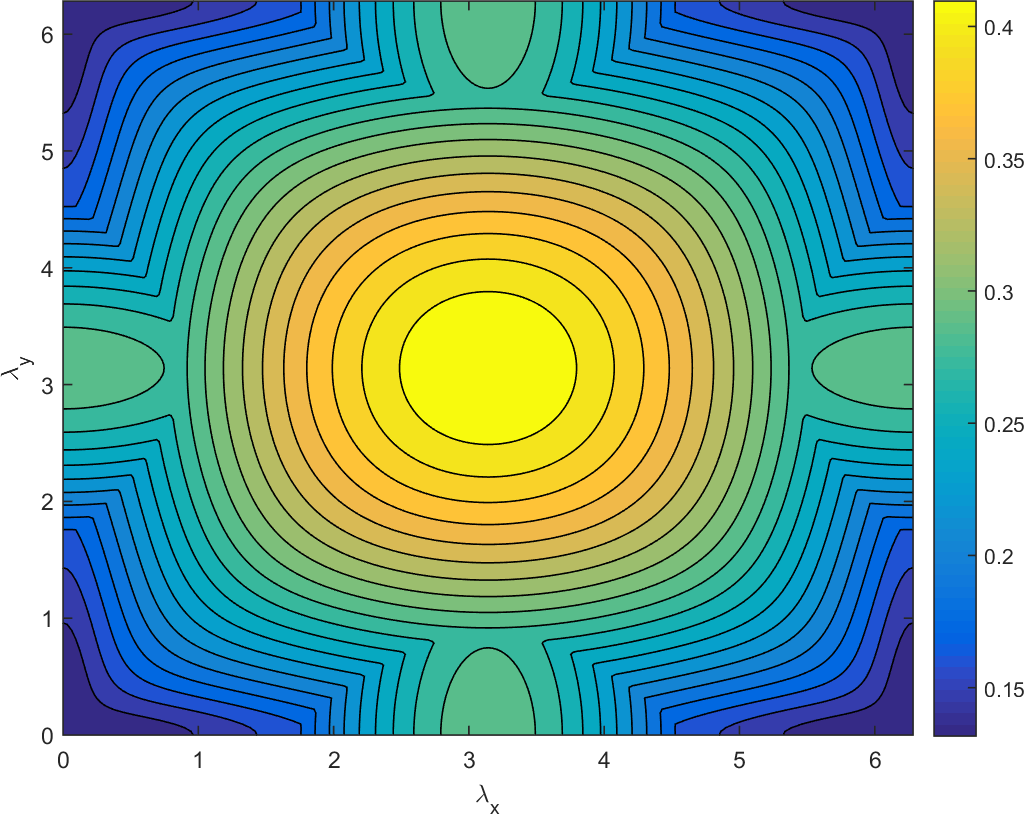
\includegraphics[width=0.975\textwidth]{figures/appendices/SI_M4S_UPWLD1_LS16_x=10_dydx=1_contour.png}
		\caption{$10^{1}$ mfp}
	\end{subfigure}
	}
	\vspace{0.5cm}
	{
	\begin{subfigure}[b]{0.485\textwidth}
		\centering
		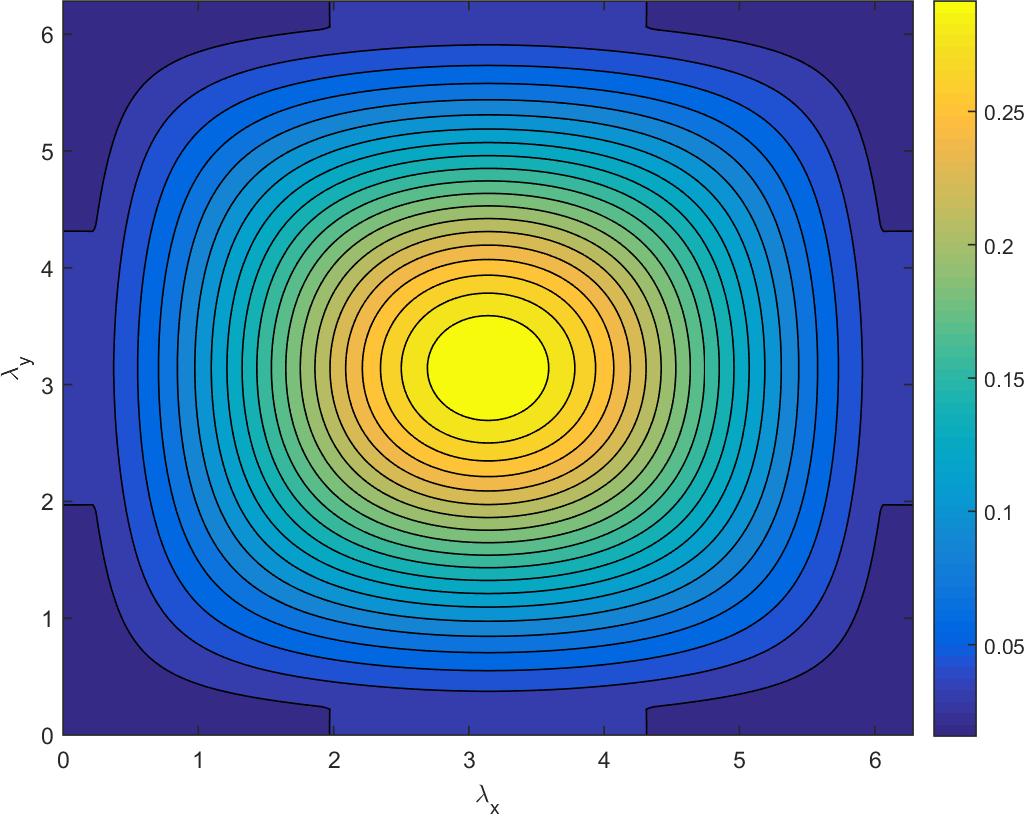
\includegraphics[width=0.975\textwidth]{figures/appendices/SI_M4S_UPWLD1_LS16_x=100_dydx=1_contour.png}
		\caption{$10^{2}$ mfp}
	\end{subfigure}
	\hfill
	\begin{subfigure}[b]{0.485\textwidth}
		\centering
		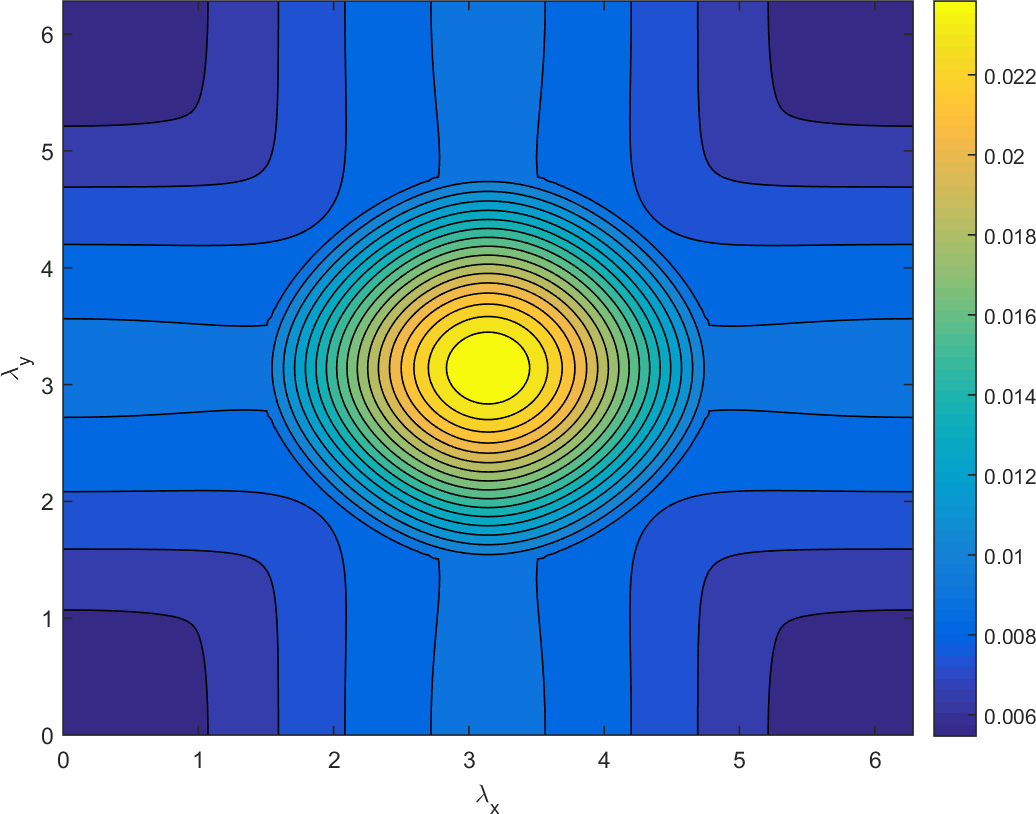
\includegraphics[width=0.975\textwidth]{figures/appendices/SI_M4S_UPWLD1_LS16_x=1000_dydx=1_contour.png}
		\caption{$10^{3}$ mfp}
	\end{subfigure}
	}
\caption{Fourier wave number distribution for different mesh optical thicknesses of a single 2D square cell with PWL basis functions and $LS_{16}$ quadrature.}
\label{fig::App_DSA_M4S_LS16}
\end{figure}